\documentclass[12pt,a4paper,bibliography=totocnumbered,listof=totocnumbered]{scrartcl}
\usepackage[ngerman]{babel}
\usepackage[utf8]{inputenc}
\usepackage{amsmath}
\usepackage{amsfonts}
\usepackage{amssymb}
\usepackage{graphicx}
\usepackage{fancyhdr}
\usepackage{tabularx}
\usepackage{geometry}
\usepackage{setspace}
\usepackage[right]{eurosym}
\usepackage[printonlyused]{acronym}
\usepackage{subfig}
\usepackage{floatflt}
\usepackage[usenames,dvipsnames]{color}
\usepackage{colortbl}
\usepackage{paralist}
\usepackage{array}
\usepackage{titlesec}
\usepackage{parskip}
\usepackage[right]{eurosym}
\usepackage[subfigure,titles]{tocloft}
\usepackage[pdfpagelabels=true]{hyperref}

\usepackage{listings}
\lstset{basicstyle=\footnotesize, captionpos=b, breaklines=true, showstringspaces=false, tabsize=2, frame=lines, numbers=left, numberstyle=\tiny, xleftmargin=2em, framexleftmargin=2em}
\makeatletter
\def\l@lstlisting#1#2{\@dottedtocline{1}{0em}{1em}{\hspace{1,5em} Lst. #1}{#2}}
\makeatother

\geometry{a4paper, top=27mm, left=30mm, right=20mm, bottom=35mm, headsep=10mm, footskip=12mm}

\hypersetup{unicode=false, pdftoolbar=true, pdfmenubar=true, pdffitwindow=false, pdfstartview={FitH},
	pdftitle={Bachelorarbeit},
	pdfauthor={Rene Zarwel},
	pdfsubject={Heterogene Microservices},
	pdfcreator={\LaTeX\ with package \flqq hyperref\frqq},
	pdfproducer={pdfTeX \the\pdftexversion.\pdftexrevision},
	pdfkeywords={Bachelorarbeit},
	pdfnewwindow=true,
	colorlinks=true,linkcolor=black,citecolor=black,filecolor=magenta,urlcolor=black}
\pdfinfo{/CreationDate (D:20110620133321)}

\newcommand{\newparagraph}[1]{\paragraph{#1}\mbox{}\\}
\newcommand{\newsubparagraph}[1]{\subparagraph{#1}\mbox{}\\}

\begin{document}

\titlespacing{\section}{0pt}{12pt plus 4pt minus 2pt}{-6pt plus 2pt minus 2pt}

% Kopf- und Fusszeile
\renewcommand{\sectionmark}[1]{\markright{#1}}
\renewcommand{\leftmark}{\rightmark}
\pagestyle{fancy}
\lhead{}
\chead{}
\rhead{\thesection\space\contentsname}
\lfoot{Heterogene Microservices}
\cfoot{}
\rfoot{\ \linebreak Seite \thepage}
\renewcommand{\headrulewidth}{0.4pt}
\renewcommand{\footrulewidth}{0.4pt}

% Vorspann
\renewcommand{\thesection}{\Roman{section}}
\renewcommand{\theHsection}{\Roman{section}}
\pagenumbering{Roman}

% ----------------------------------------------------------------------------------------------------------
% Titelseite
% ----------------------------------------------------------------------------------------------------------
\thispagestyle{empty}
\begin{center}
	
\includegraphics[scale=0.5]{Bilder/Hochschule_Muenchen_Logo.png}\\
	\vspace*{2cm}
	\Large
	\textbf{Fakultät für Informatik und Mathematik 07}\\
	\vspace*{2cm}
	\Huge
	\textbf{Bachelorarbeit}\\
	\vspace*{0.5cm}
	\large
	über das Thema\\
	\vspace*{1cm}
	\textbf{Heterogene Microservices}\\
	\vspace*{2cm}
	
	\vfill
	\normalsize
	\newcolumntype{x}[1]{>{\raggedleft\arraybackslash\hspace{0pt}}p{#1}}
	\begin{tabular}{x{6cm}p{7.5cm}}
		\rule{0mm}{5ex}\textbf{Autor:} & René Zarwel\newline zarwel@hm.edu \\ 
		\rule{0mm}{5ex}\textbf{Prüfer:} & Prof. Dr. Hammerschall \\ 
		\rule{0mm}{5ex}\textbf{Abgabedatum:} & XX.XX.XX\\ 
	\end{tabular} 
\end{center}
\pagebreak

% ----------------------------------------------------------------------------------------------------------
% Abstract
% ----------------------------------------------------------------------------------------------------------
\setcounter{page}{1}
\onehalfspacing
\titlespacing{\section}{0pt}{12pt plus 4pt minus 2pt}{2pt plus 2pt minus 2pt}
\rhead{KURZFASSUNG}
\section{Kurzfassung}
Insert Abstract Here

\vspace{-1,2em}
\titlespacing{\section}{0pt}{12pt plus 4pt minus 2pt}{-6pt plus 2pt minus 2pt}
\section*{Abstract}
Insert Abstract Here
\pagebreak

% ----------------------------------------------------------------------------------------------------------
% Verzeichnisse
% ----------------------------------------------------------------------------------------------------------
% TODO Typ vor Nummer
\renewcommand{\cfttabpresnum}{Tab. }
\renewcommand{\cftfigpresnum}{Abb. }
\settowidth{\cfttabnumwidth}{Abb. 10\quad}
\settowidth{\cftfignumwidth}{Abb. 10\quad}

\titlespacing{\section}{0pt}{12pt plus 4pt minus 2pt}{2pt plus 2pt minus 2pt}
\singlespacing
\rhead{INHALTSVERZEICHNIS}
\renewcommand{\contentsname}{II Inhaltsverzeichnis}
\phantomsection
\addcontentsline{toc}{section}{\texorpdfstring{II \hspace{0.35em}Inhaltsverzeichnis}{Inhaltsverzeichnis}}
\addtocounter{section}{1}
\tableofcontents
\pagebreak
\rhead{VERZEICHNISSE}
\listoffigures
\pagebreak
\listoftables
%\pagebreak
\renewcommand{\lstlistlistingname}{Listing-Verzeichnis}
{\labelsep2cm\lstlistoflistings}
\pagebreak

% ----------------------------------------------------------------------------------------------------------
% Abkürzungen
% ----------------------------------------------------------------------------------------------------------
\section{Abkürzungsverzeichnis}
\begin{acronym}[OSGi] % längste Abkürzung steht in eckigen Klammern
	\setlength{\itemsep}{-\parsep} % geringerer Zeilenabstand
	\acro{API}{Programmierschnittstelle}
\end{acronym}
\newpage

% ----------------------------------------------------------------------------------------------------------
% Inhalt
% ----------------------------------------------------------------------------------------------------------
% Abstände Überschrift
\titlespacing{\section}{0pt}{12pt plus 4pt minus 2pt}{-6pt plus 2pt minus 2pt}
\titlespacing{\subsection}{0pt}{12pt plus 4pt minus 2pt}{-6pt plus 2pt minus 2pt}
\titlespacing{\subsubsection}{0pt}{12pt plus 4pt minus 2pt}{-6pt plus 2pt minus 2pt}

% Kopfzeile
\renewcommand{\sectionmark}[1]{\markright{#1}}
\renewcommand{\subsectionmark}[1]{}
\renewcommand{\subsubsectionmark}[1]{}
\lhead{Kapitel \thesection}
\rhead{\rightmark}

\onehalfspacing
\renewcommand{\thesection}{\arabic{section}}
\renewcommand{\theHsection}{\arabic{section}}
\setcounter{section}{0}
\pagenumbering{arabic}
\setcounter{page}{1}

% ----------------------------------------------------------------------------------------------------------
% Einleitung
% ----------------------------------------------------------------------------------------------------------
\section{Einleitung}

\pagebreak
% ----------------------------------------------------------------------------------------------------------
% Grundlagen
% ----------------------------------------------------------------------------------------------------------
\section{Microservices}

\bigquote{Do One Thing and Do It Well}{Douglas McIlroy (A Quarter Century of Unix)}

Diesem Grundsatz aus der Unix Philosophie folgt auch die Microservice Architektur. Sie bietet einen Ansatz zur Modularisierung von Software. Doch im Gegensatz zur konventionellen Modularisierung von großen Systemen, sind die sogenannten Microservices eigene Programme\cite[10]{Wolff2015}, die über eine einheitliche Schnittstelle, wie z.~B. \ac{REST} oder Messaging, kommunizieren. Ein einzelner Service ist dabei relativ klein, weitgehend entkoppelt und  übernimmt nur eine kleine Aufgabe.\\
Doch ist dies nur ein Aspekt des Entwurfsmusters. Die Abbildung \ref{MicroservicesVorteile} zeigt hierzu die wesentlichen Vorteile einer Microservice Architektur.

\image[MicroservicesVorteile.pdf]{MicroservicesVorteile}{Vorteile Microservices}{Wesentliche Vorteile von Microservices\cite[12]{Wolff2015}}

\begin{description}[leftmargin=!,labelwidth=\widthof{\bfseries Ergänzung Legacy-Systeme}]
	\item[Starke Modularisierung] 
	 	Durch die strikte Trennung der einzelnen Services in eigene Programme, schleichen sich kaum unerwünschte Abhängigkeiten unter den Modulen ein.
	\item[Ersetzbarkeit]
		Solange die Schnittstelle eines Services gleich bleibt, kann dieser einfach ersetzt werden. Dabei muss er weder die Code-Basis noch die Technologie des bestehenden Services verwenden.
	\item[Nachhaltige Entwicklung] 
		Mit der starken Modularisierung und der Ersetzbarkeit können technische Schulden vermieden und so eine nachhaltige Entwicklung geschaffen werden.
	\item[Effiziente Skalierung]
		Durch die starke Trennung lassen sich die einzelnen Module unabhängig voneinander skalieren.
	\item[Continuous Delivery]
		Dank der kleineren Services lässt sich einfacher eine Continuous-Delivery-Pipeline aufbauen. So können einzelne Services schneller in die Produktion gebracht werden, wodurch sich die Time-To-Market Zeit verringert. 
	\item[Technologie Freiheit]
		Einzelne Services können unterschiedliche Technologien verwenden. Es besteht dabei keine Einschränkung auf eine Programmiersprache oder Plattform.
\end{description}

Besonders die technologische Freiheit ist an dieser Stelle interessant. Durch die Aufteilung in einzelnen Services, können für jeden Microservice unabhängig die Programmiersprache und Frameworks gewählt werden. So lassen sich neue Technologien in einem Service erproben, ohne dass andere Services davon betroffen sind. Dies senkt das Risiko für die Einführung neuer Technologien und die Kosten bleiben kalkulierbar\cite[13]{Wolff2015}, da nur in einem kleinen Rahmen eingeführt und getestet wird.\\
Die Technologie-Entscheidung könnte somit auf die kleine Teilaufgabe, die der Service übernimmt, reduziert werden. Aber auch die Fähigkeiten des Entwickler-Teams spielen eine Rolle. So kann z.~B. für das eine Team NodeJS gewählt werden, da überwiegend Javascript Entwickler vertreten sind, und für das andere Team Spring, da dieses hauptsächlich Java beherrschen.

\subsection{Microservice Frameworks}\label{Microservice_Frameworks}

Ein Microservice Framework soll die Erstellung eines Services vereinfachen. Es unterstützt den Entwickler bei sich wiederholenden Tätigkeiten, wie z.~B. der Erstellung eines \ac{REST}-Endpunktes, und bringt viele häufig benötigte Funktionen mit. Dies könnte z.~B. eine Authentifizierung oder Caching sein.\\
Dabei ist es darauf ausgelegt, möglichst schnell Ergebnisse zu erzielen und einen lauffähigen Microservice zu erstellen. Dies ist wichtig, da aufgrund der Vielzahl von Services die Erstellung eines einzigen nicht zu komplex sein sollte und der Fokus auf der Geschäftslogik liegt. 

Dank der Technologiefreiheit kann für jeden Service ein eigenes Framework gewählt werden. Dabei stellt sich die Frage, welches für die Lösung der Teilaufgabe am besten geeignet ist. \\
Da es einen Rahmen für die Entwicklung zur Verfügung stellt und die Programmiersprache vorgibt, ist diese Entscheidung maßgeblich für den weiteren Entwurf des Services. Aus diesem Grund sollte die Wahl nicht gänzlich unbedacht sein. Auch wen mit der Ersetzbarkeit die Hürde zum Austausch gering ist, bedeutet ein Fehlschlag mitunter mehrere Wochen vergeudetet Entwicklungszeit.

Um das richtige Framework zu finden, müssen die Anforderungen an den Service festgelegt sein. Nur wenn es diese erfüllt, macht eine Umsetzung mit dem Framework Sinn. Somit sollten bei der Bewertung eines Frameworks die Erfüllung der spezifischen Serviceanforderungen geprüft werden.\\
Welche Anforderungen ein Service zu erfüllen hat, ergibt sich aus der Aufgabe, die mit dem Service umgesetzt werden soll. Dies können sowohl fachliche Aufgaben, wie eine Kundenverwaltung, oder technische, wie das Sammeln von Log-Daten der weiteren Services, sein.\\
Aus der Architektur ergibt sich die Aufteilung der Aufgaben. Dabei ist es wichtig, dass bei Änderungen und neuen Features nur ein Service angepasst werden muss. Hierzu ist es essentiell, dass jeder Service eine fachliche bzw. technische Einheit bildet.\\
Durch die Anforderungen des Gesamtsystems, die hauptsächlich vom Auftraggeber vorgegeben sind, ergibt sich die Architektur. Dieser Weg von den Anforderungen bis zur Wahl der passenden Frameworks ist in Abbildung \ref{FrameNeeds} nochmals dargestellt.
    
\image[FrameNeeds.pdf][width=0.3\linewidth]{FrameNeeds}{Anforderungen und Frameworks}{Der Weg von den Anforderungen zu den passenden Frameworks für die Services}
 
Aus diesem Zusammenhang wird ersichtlich, dass sich nur dann die passenden Serviceanforderungen für die Bewertung eines Frameworks ergeben, wenn die Architektur den Anforderungen entspricht. Bevor man ein Framework bewerten kann, muss somit die Qualität der Architektur bewiesen sein. Nur dann kann man sicher gehen, dass der richtige Maßstab für die Wahl des passenden Frameworks angelegt wird.

Es bietet sich somit an, die Bewertung von Frameworks an die Qualitätsbewertung von Softwarearchitektur anzulehnen. So kann gewährleistet werden, dass die Serviceanforderungen in direkter Beziehung zu den Anforderungen des Gesamtsystems stehen und die Wahl des passenden Frameworks nachvollziehbar bleibt.
 
\pagebreak
\section{Qualitätsbewertung von Softwarearchitektur}\label{Qualitätsbewertung_Softwarearchitektur}

\bigquote{You cannot control what you cannot measure}{Tom DeMarco (Controlling Software Projects)}

Die Aussage beschreibt sehr gut, dass ein IT-Projekt besser auf die Projektziele
zusteuern kann, wenn Messwerte erhoben werden. Diese lassen sich z.~B. in Diagrammen sehr gut darstellen und können zumeist einfach sowie unmissverständlich interpretiert werden. Neben dem aktuellen Projektstatus lassen sich so auch Trends erkennen. Diese helfen dabei rechtzeitig Abweichungen festzustellen und gegebenenfalls korrigierende Maßnahmen einzuleiten\cite{Starke2015}. Auch wenn \citeauthor{DeMarco2009} \citeyear{DeMarco2009} seine Aussage relativiert hat\cite{DeMarco2009}, bleibt sie in Bezug auf die Softwarearchitektur stimmig.
Gerade bei einem so entscheidendem Punkt, wie der Architektur, ist es wichtig frühzeitig
Risiken und Qualitätsabweichungen festzustellen. Die Architektur ist ein sehr kritischer
und wesentlicher Bestandteil im Entwicklungsprozess von einer Software. Ihrer Beschaffenheit nach,
kann sie nur schwer und mit hohen Kosten verändert werden.
Durch Zeit- und Kostendruck wird dies leider in der Praxis häufig erst in späten Entwicklungsphasen durchgeführt. 
In einem sogenannten \enquote{Audit} oder \enquote{Review} werden bereits produktiv laufende Systeme bewertet\cite{Starke2015}.
Sollten sich hier starke Abweichungen gegenüber den Anforderungen zeigen, kann sich dies zu einem großen Problem 
avancieren, hohe Kosten verursachen und Kunden verärgern.
Aus diesem Grund ist die Qualität einer Architektur sehr entscheidend und sollte stichhaltig nachgewiesen sein.
Um sie zu bestimmen und Restrisiken minimiert zu können, gibt es Methoden zur Qualitätsbewertung 
von Softwarearchitektur. Neben diesem Ziel gibt es noch weitere positive Auswirkungen, die für den Einsatz der Architekturbewertung sprechen. (Siehe Bild \ref{Architekturbewertung})

\image[Architekturbewertung.pdf][width=0.7\linewidth]{Architekturbewertung}{Ziele Architekturbewertung}{Allgemeine Ziele von Architekturbewertung.}

Die Bewertung kann sich dabei auf die im Softwareprojekt entstehenden Artefakte stützen. Beispielsweise sind
Anforderungen, Architekturen, Diagramme, Quellcode und andere Dokumente zu nennen. Diese Artefakte können dabei quantitativ 
oder qualitativ bewertet werden. So kann z.~B. der Quellcode mittels Metriken quantitativ, d.~h. in reinen Zahlen, bewertet werden. Dies lässt sich meist einfach und automatisiert, siehe SonarQube\footnote{\url{https://www.sonarqube.org}}, erfassen und kann sehr gut reproduziert sowie verglichen werden. Der Einsatz sollte jedoch gut überlegt sein, damit nicht ziellos gemessen wird.
Andere Artefakte entziehen sich dieser Bewertung und können nur auf ihre Güte hin, also qualitativ, bewertet werden. Diese, teils auch subjektiven, Bewertungen setzen einen größeren Aufwand voraus und lassen sich schwer vergleichen.  
Zu letzterem zählt die Softwarearchitektur.     

\subsection{Qualitätsmerkmale der Softwarearchitektur}

Auch bei der Architekturbewertung sind die Anforderungen das Fundament. Sie charakterisieren die 
gewünschten Eigenschaften eines Systems\cite{Starke2015}.
Bei der Softwarearchitektur gibt es eine Vielzahl an Qualitätsmerkmale anhand derer Anforderungen bestimmt und definiert werden können\cites{Starke2015}{Clements2000}:

\begin{description}[leftmargin=!,labelwidth=\widthof{\bfseries Konzeptuelle Integrität}]
	\item[Funktionalität] 
	Mit der Funktionalität wird bestimmt, ob die funktionalen Anforderungen nicht nur vollständig erfüllt werden, sondern auch richtig und angemessen umgesetzt sind.
	\item[Zuverlässigkeit] 
	Aus der Zuverlässigkeit ergibt sich die Fähigkeit eines Systems, die Funktion innerhalb einer Zeitspanne umzusetzen und
	dabei auf etwaige Fehler zu reagieren bzw. diese zu verhindern.
	\item[Leistung] 
	Die Leistung (Performance) gibt an, wie schnell das System reagiert und wie viele Eingaben pro Zeiteinheit verarbeitet werden können. Diese Anforderungen
	lassen sich meist über Benchmarks testen.
	\item[Flexibilität] 
	Eine Architektur ist flexibel, wenn sie angepasst und erweitert werden kann, ohne dabei das gesamte Konstrukt zu zerstören.
	\item[Übertragbarkeit] 
	Durch die Übertragbarkeit lässt sich das System auch unter verschiedensten Voraussetzungen betreiben. (Hard- und Softwareumgebungen) 
	\item[Unterteilbarkeit]
	Die Unterteilbarkeit ermöglicht eine einfache Aufteilung in Teilsysteme. So können einzelne Teile unabhängig entwickelt oder sogar betrieben werden.
	\item[Konzeptuelle Integrität] 
	Das Konzept sollte sich auf allen Ebenen widerspiegeln und sich durch ein einheitliches Design präsentieren. Ähnliche Dinge sollen dabei in ähnlicher Art und Weise gelöst werden. 
	\item[Machbarkeit] 
	Es muss möglich sein, das System mit vorhandenen Ressourcen (Technologie, Budget, usw.) umzusetzen.
\end{description}

Diese Aufzählung stellt hierbei eine Auswahl an verschiedenen allgemeinen Qualitätsmerkmalen dar und erhebt dabei keinen Anspruch auf Vollständigkeit.

\subsection{Soll-Ist-Vergleich}
\
Mit den Anforderungen kann ein Soll-Ist-Vergleich anhand der Artefakte durchgeführt werden. Jede einzelne Anforderung wird dabei mit Plänen, Dokumentation oder Modellen verglichen und bewertet. D.~h. es wird geprüft, ob das geplante System den Anforderungen entsprechen wird. Wichtig ist, dass die geforderten Eigenschaften möglichst feingranular sind. Je detaillierter die Anforderungen vorliegen, desto geringer ist das Restrisiko einzelne Punkte zu vergessen oder unscharf zu bewerten.
  
Das Ergebnis dieser Prüfung kann folgendermaßen aussehen\cite{Starke2015}:

\begin{description}[leftmargin=!,labelwidth=\widthof{\bfseries Soll $=$ Is}]
	\item[Soll $=$ Ist] 
	Das Soll wird erfüllt und die Architektur besitzt alle geforderten Eigenschaften.
	\item[Soll $\approx$ Ist] 
	Das Soll wird nur teilweise erreicht und es werden Kompromisse geschlossen. (Verbesserung einzelner Anforderungen)
	\item[Soll $\neq$ Ist] 
	Das Soll wird nicht erfüllt und es ergibt sich ein Risiko für das System
\end{description}

Die Architekturbewertung ist somit ein relativer Vergleich in Hinblick auf spezifische 
Kriterien und liefert keine absolute Aussage über die Qualität. Vielmehr identifizieren sich aus einer Architekturbewertung Risiken, die die Architekturentscheidungen in der Entwurfsphase mit sich gebracht haben. 

Diesen Ansatz verfolgt auch \ac{SAAM}. Das \ac{SEI}, eine US-Bundeseinrichtung für die Verbesserung von Software-Engineering Praktiken, hat mit dieser Methode den Grundstein der Architekturbewertung gelegt.
Viele der heute bekannten 
Methoden basieren auf der \ac{SAAM} und erweitern diese um spezielle Sichten oder fokussieren sich auf ein spezielles Qualitätsmerkmal. Mit der \ac{ATAM} wurde die \ac{SAAM} von der \ac{SEI} weiterentwickelt und stellt heute die führende Methode zur Architekturbewertung dar\cite{ATAM_SEI}.

\subsection{\acf*{ATAM}}

Im folgenden Abschnitt wird \ac{ATAM} genauer vorgestellt. Das Ziel dieser Bewertungsmethode ist nicht eine exakte Vorhersage über die 
zu erwartende Qualität der Software zu treffen. Das ist nahezu unmöglich bei der frühen Entwurfsphase, da noch nicht genügend Informationen 
vorliegen. Vielmehr soll der Blick auf einzelne Qualitätsmerkmale und dessen Abhängigkeit zu gewissen Architektur-Entwurfsentscheidungen geschärft 
werden\cite{Clements2000}. Mit diesem Wissen können einzelne Entscheidungen überdacht, genauer modelliert oder angepasst werden, um das gewünschte 
Qualitätsziel zu erreichen. Darüber hinaus wird auch die Dokumentation der Architektur verbessert, da alle Qualitätsaspekte genauer untersucht werden.

Das Ziel von \ac{ATAM} ist eine Dokumentation von Risiken (Risks), Sensitivitätspunkte (sensitivity points) und Kompromisspunkte(tradeoff points), die durch eine genauere Analyse der Architektur\cite{Clements2000}
ermittelt werden konnten. 
Risiken stellen nicht getroffene Architekturentscheidungen oder Eigenschaften der Architektur,die nicht vollständig
verstanden wurden, dar. So kann z.~B. der verwendete Datenbanktyp noch ungeklärt oder die Auswirkungen einer zentral geführten Komponente unklar sein.

Sensitivitätspunkte sind starke Abhängigkeiten messbarer Qualitätsmerkmale. Diese beziehen sich auf die Auslegung von einzelnen Komponenten der Architektur. Ein Beispiel für Sensitivitätspunkte ist ein Engpass zwischen zwei Modulen. D.~h. wenn der Kommunikationskanal zweier Module, wovon mindestens eins essenziell für das Gesamtsystem ist, zu gering ausgelegt wurde, dann kann dieser für einen niedrigen Durchsatz des gesamten Systems verantwortlich sein. In anderen Worten beeinflusst die Dimensionierung einer einzelnen Komponente direkt das Gesamtsystem, was einen Sensitivitätspunkt darstellt.

Zusätzlich deckt der Kompromisspunkt Sensitivitätspunkte auf, die sich entgegen wirken.
Würde man z.~B. den zuvor genannten Engpass breiter auslegen, kann unter Umständen dies die Zuverlässigkeit des Gesamtsystems verschlechtern. Ein angebundenes Modul verwirft möglicherweise bei einer starken Belastung einige Anfragen, wodurch ein korrektes Ergebnis nicht mehr garantiert werden kann. So wirken sich diese beiden Sensitivitätspunkte entgegen und es muss ein Kompromiss gebildet werden.  
 
Mit den Risiken, Sensitivitäts- und Kompromisspunkten kann die Architektur mit gezielteren Analysen, Erstellung von Prototypen und weiteren Entwürfen stark verbessert 
werden. 

Die Grundvoraussetzung zum Erreichen dieses Zieles ist eine detaillierte Definition der Qualitätsanforderungen und eine genaue Spezifikation der Architektur sowie
dessen zugrunde liegenden Entscheidungen\cite{Clements2000}. In der Praxis ist es leider nicht unüblich, dass Ziele und Architekturdetails noch unklar oder mehrdeutig sind. Aus diesem Grund ist ein wichtiges Ziel von \ac{ATAM} auch dies genauer zu definieren und eindeutig festzuhalten. Um die Erreichung sämtlicher Ziele zu unterstützen, ist \ac{ATAM} in 
mehrere Phasen aufgeteilt. Bild \ref{ATAMPhasen} gibt hierzu einen Überblick.

\image[ATAM-Phasen.pdf]{ATAMPhasen}{Phasen von ATAM}{Phasen der Architekturbewertung nach ATAM\cite{Starke2015}}

\subsubsection{Vorbereitung}
\
Das Fundament der Bewertung stellen die Qualitätsanforderungen dar. Diese können nur lückenlos bestimmt werden, wenn alle maßgeblich vom Projekt betroffenen Personen involviert sind. In der Vorbereitungs-Phase müssen alle wichtigen Stakeholder identifiziert werden. Neben dem Kunden bzw. Auftraggeber selbst, kann dies z.~B. der Benutzer, Administrator oder Tester sein. Dabei müssen jene Personen nicht direkt in den Prozess miteinbezogen werden. Es reicht schon einen Vertreter, meist aus dem Management, zu bestimmen oder die Wünsche und Ziele vorher genau zu ermitteln. In der Regel werden nur wenige Stakeholder, meist Personen aus dem Management und der Projektleitung\cite{Starke2015}, direkt zur Architekturbewertung eingeladen. Zu viele Personen würden den Prozess, durch Diskussionen und Abschweifungen, nur verlangsamen und ineffektiv gestalten.
\subsubsection{Kickoff-Phase}
\newparagraph{Bewertungsmethode (ATAM) vorstellen}
\
Im ersten Schritt soll die Bewertungsmethode vorgestellt und dessen Ziele verdeutlicht werden. Nicht jeder Stakeholder ist regelmäßig in eine Architekturbewertung involviert. So muss klar gestellt werden, welche Bedeutung das Architektur- und Qualitätsziel hat\cite{Starke2015}. Des Weiteren sollte hervorgehoben werden, dass es bei der qualitativen Architekturbewertung um das Aufdecken von Risiken sowie um mögliche Maßnahmen geht. Es sollte nicht Ziel sein, Noten für die Architektur zu vergeben. Insbesondere sollte die Präsentation folgende Punkte enthalten\cite{Clements2000}:

\begin{itemize}[]
	\item Eine Kurze Beschreibung von ATAM und dessen Ablauf
	\item Methoden zur Analyse sollten erklärt werden
	\item Das Ziel und die Ergebnisse der Evaluation
\end{itemize}

\newparagraph{Qualitätsziel vorstellen}
\
Die Qualitätsanforderungen werden wesentlich vom Auftraggeber bestimmt. Aus diesem Grund sollte er auch diese vorstellen und dabei genau erläutern, was die Gründe für die Entwicklung sind und wie das System in die fachlichen Unternehmensprozesse eingeordnet werden soll. Selbst wenn die Ziele bereits in einem Anforderungsdokument erfasst wurden, ist es wichtig, die aktuelle Sichtweise des Auftraggebers zu begreifen. Zudem sind Zielformulierungen aus den Anforderungsdokumenten, meist von Systemanalytikern, gründlich gefiltert worden\cite{Starke2015}. So können Teilnehmer Rückfragen stellen und Aha-Erlebnisse auslösen.

\newparagraph{Architektur erläutern}
\
In dieser Phase wird vom Softwarearchitekten die Architektur vorgestellt. Dabei wird nicht nur das eigentliche System erläutert, sondern es sollte auch der gesamte Kontext mit einbezogen werden\cite{Starke2015}. Es beinhaltet Nachbarsysteme oder Plattformen mit denen das System in Verbindung steht. Eine angemessene Detailtiefe spielt dabei auch eine Rolle. Was angemessen ist, hängt in erster Linie von den vorhandenen Informationen (Dokumente, Diagramme, usw.) und der verfügbaren Zeit ab. Dies stellt einen wesentlichen Punkt in der Bewertung dar\cite{Clements2000}, da nur die bereitgestellten Informationen in die Analyse mit einbezogen werden können. Je mehr vorhanden ist, desto tiefer und detaillierter kann die Bewertung durchgeführt werden. Wichtige und benötigte Dokumente oder Entscheidungen zur Architektur sollten unbedingt vor der Evaluation erstellt worden sein.
Die Präsentation der Architektur sollte hier folgende Informationen umfassen\cites{Clements2000}{Starke2015}:

\begin{itemize}[]
	\item Bausteine der oberen Abstraktionsebene
	\item Ausgewählte Laufzeitsichten wichtiger Use-Cases
	\item Technische Einschränkungen, wie Betriebssystem, Hardware oder Middleware
	\item Weitere Systeme mit denen dieses zusammenhängt 
\end{itemize}
\subsubsection{Bewertungsphase}
\newparagraph{Architekturansätze identifizieren}
\
Aus der vorangegangenen Information können nun Architekturentscheidungen identifiziert werden, die zur Erfüllung spezieller Qualitätsanforderungen dienen. Es ist zu klären, wie die Architektur, strukturell oder konzeptionell, die wesentlichen Probleme oder Herausforderungen löst. Die treibenden und prägenden Architekturansätze werden dabei von den Architekten hervorgehoben und dienen der Ergänzung des voraufgegangenem Überblicks\cite{Starke2015}.
Die Erfüllung der kritischen Anforderungen von der Architektur wird so sichergestellt.

\newparagraph{Bildung eines Qualitätsbaumes (Quality Utility Tree)}
\
In dieser Phase werden alle Stakeholder aktiv. Sie identifizieren und verfeinern die wichtigsten Qualitätsanforderungen des Systems. Wichtig dabei ist den Fokus nicht auf die wesentlichen Anforderungen zu verlieren und sich in Feinheiten zu verstricken\cite{Clements2000}. Damit dies gelingen kann, wird ein Qualitätsbaum erstellt.
So werden die wesentlich geforderten Anforderungen, z.~B. in einem Brainstorming, erfasst und anschließend in Baum-Form angeordnet. Die globalen Anforderungen stehen auf der linken Seite und werden nach rechts hin verfeinert. Bild \ref{Qualitaetsbaum} stellt ein Beispiel für einen solchen Qualitätsbaum dar. 

\image[BeispielQualitaetsbaum.pdf]{Qualitaetsbaum}{Beispiel Qualitätsbaumes}{Beispiel eines Qualitätsbaums.}

Anschließend werden zu den Qualitätsanforderungen Szenarien erstellt. Diese bilden einen wichtigen Bestandteil der Bewertungsmethode. Sie dienen dazu, die Anforderungen genauer zu definieren und den Stakeholdern somit näher zu bringen. Dabei muss die Formulierung eines Szenarios möglichst konkret sein und ein Beispiel darstellen, wie sich das System in einer bestimmten Situation verhält. Ein Szenario sollte folgende Informationen umfassen\cite{Starke2015}:

\begin{description}[leftmargin=!,labelwidth=\widthof{\bfseries Systembestandteil}]
	\item[Auslöser] Welcher spezifischer Stimulus löst das Szenario aus.
	\item[Quelle] Woher stammt der Auslöser. Z. B. intern, extern, Benutzer, Administrator usw.
	\item[Umgebung] Welcher Bestandteil des Systems ist betroffen.
	\item[Antwort] Wie reagiert das System auf den Auslöser.
	\item[Metrik] Wie kann die Antwort gemessen oder bewertet werden.
\end{description}

Die Szenarien sind nicht nur eine genauere Definition der Anforderungen. Auch helfen sie den Projektbeteiligten dabei, die Qualitätseigenschaften genauer zu verstehen, da sie weniger abstrakt sind und konkrete Anwendungsfälle enthalten. Ein, um Szenarien erweiterter Qualitätsbaum, ist in Bild \ref{QualitaetsbaumSzenarien} dargestellt.

\image[BeispielQualitaetsbaumMitSzenarien.pdf]{QualitaetsbaumSzenarien}{Qualitätsbaum und Szenarien}{Qualitätsbaum mit einzelnen Szenarien erweitert}

Zuletzt werden den Szenarien Prioritäten zugeordnet, so dass der Fokus zuerst auf kritische Anforderungen steht. Auch ist der Bewertungs-Workshop meist zeitlich begrenzt und somit wird sichergestellt, dass die Nichterfüllung essentieller Qualitätsanforderungen schnell zu einem Abbruch führt. Es kann durch eine einfache Skala mit wenigen Prioritäten erreicht werden, z.~B. A = hoch, B = mittel und C = weniger wichtig.

\newparagraph{Architekturansätze analysieren}
\
Anhand der Prioritäten kann nun die eigentliche Analyse beginnen. In kleineren Gruppen, zusammen mit den Architekten oder Entwicklern, werden die Szenarien genauer untersucht und zugehörige Architekturansätze erläutert.
So kann z.~B. mittels eines Walkthrough genau aufgezeigt werden, wie einzelne Komponenten zur Erreichung des Ziels interagieren und welche Entwurfsentscheidungen unterstützen\cite{Starke2015}. Dabei sollten folgende Fragen geklärt werden: 

\begin{itemize}
	\item Wie wird das Szenario in der Architektur umgesetzt?
	\item Warum wurde dieser Architekturansatz gewählt?
	\item Gibt es Kompromisse, die gemacht wurden?
	\item Werden andere Qualitätsmerkmale davon beeinflusst?
	\item Gibt es Risiken die damit verbunden sind?
	\item Wird die Entscheidung von Analysen, Untersuchungen oder Prototypen unterstützt?
\end{itemize}

Die Analyse ist dabei nicht auf diese Fragen beschränkt. Sie bieten lediglich einen Startpunkt für eine Diskussion, um potentielle Risiken, Sensitivitäts- oder Kompromisspunkte zu finden. An dieser Stelle gibt es leider kein Patentrezept oder ein spezifisches Vorgehen, um das Erfüllen der Qualitätsanforderung zu bestimmen. Viel mehr wird von den Teilnehmern ein analytisches und systematisches Denken verlangt. Im Fokus muss hierbei stehen, dass eine Verbindung zwischen der Architekturentscheidung und der Anforderung geschaffen wird, die sie erfüllen soll.

\subsubsection{Abschlussphase}
\
Am Ende wird das Ergebnis den Stakeholdern präsentiert. Es muss nicht zwangsläufig nur durch eine Präsentation dargestellt, sondern kann auch um einen detaillierten Berichte ergänzt werden. Sämtliche Phasen der Bewertung und dessen Ergebnisse können so noch einmal rekapituliert werden und bilden die Basis zur Definition von eventuell benötigten Maßnahmen.

Die durch \ac{ATAM} gefundenen Risiken und die daraus resultierenden Maßnahmen können auch Änderungen an der Architektur darstellen. Daher bietet sich \ac{ATAM} auch zum iterativen Einsatz an. Mit ersten Entwürfen einer komplexen Architektur kann überprüft werden, ob die Entscheidungen den richtigen Weg einschlagen und wichtige Anforderungen von Beginn an mit einbezogen werden. So bildet sich Schrittweise eine detaillierte Architektur unter gut dokumentierter Berücksichtigung der Qualitätsanforderungen. 

Einen anderen Ansatz verfolgt die \ac{SAEM} Methode. Diese betrachtet die Softwarearchitektur als finales Produkt der Entwurfsphase und versucht mittels dem ISO/IEC 25010\footnote{
	In der ursprünglichen Veröffentlichung von \ac{SAEM} wurde das ISO/IEC 9126-1 Modell verwendet. Die ISO/IEC 9126-1 wurde 2011 durch die ISO/IEC 25010 ersetzt.
}
Qualitätsmodell die Qualität der Architektur festzustellen.


\subsection{\acf*{SAEM}}

Im Gegensatz zu \ac{ATAM} ist \ac{SAEM} weniger bekannt und erprobt\cite{IEEE_TSE2002}. Sie zielt darauf ab die Qualität der Softwarearchitektur selbst festzustellen. Nicht nur weil Fehler in der Architektur schwer zu beheben sind, sondern diese auch direkt einen Einfluss auf die Qualität und Kapazitäten des Systems haben\cite{Duenas1998}. Dies trifft besonders auf die nicht-funktionalen Anforderungen, wie Wartbarkeit, Skalierbarkeit oder Effizienz, zu.

Wie beim finalen System ist die direkte Messung am Produkt eine objektive und sehr effektive Evaluation der Qualität. Um dies zu erreichen, müssen Qualitätsanforderungen definiert und ein Prozess zur Überprüfung dieser  geplant, implementiert und kontrolliert werden\cite{Duenas1998}. \ac{SAEM} versucht dies mittels eines Qualitätsmodells auf die Softwarearchitektur abzubilden und stellt Methoden sowie Metriken für die Evaluation bereit. 

\subsubsection{Spezifikation Qualität}
\
Das Qualitätsmodell von \ac{SAEM} baut dabei auf dem Modell der ISO/IEC 25010 auf. Jenes teilt die Qualität in 8 Kategorien und weitere Unterkategorien auf\cite{ISOIEC25010}. Anhand derer kann die Qualität der Softwarearchitektur spezifiziert werden, indem man diesen Architekturanforderungen zuordnet.

\image[ISO25010.pdf]{ISO25010Modell}{Qualitätsmodell der ISO/IEC 25010}{Qualitätsmodell der ISO/IEC 25010\cite{ISOIEC25010}}

Hierzu wird im ersten Schritt die externe Qualität bestimmt. Diese basiert auf messbaren Metriken unter Nutzungsbedingungen und werden vom Nutzer sowie den Architekten definiert\cite{Duenas1998}. So sollten, für alle Qualitätskategorien, Anforderungen an die Architektur ausgewählt und optimale bzw. zulässige Werte bestimmt werden. Ein Beispiel hierfür ist die Reaktionszeit auf Anfragen. 
Mittels der externen Qualität können die Architekten die interne Qualität bestimmen. Diese sind Anforderungen, die zur Erreichung und Zufriedenstellung des Ziels benötigt werden. Im Unterschied zu externen Anforderungen werden diese nicht durch die Nutzung bestimmt, sondern beziehen sich auf intrinsische Eigenschaften, wie z.~B. Modularität oder Komplexität\cite{Duenas1998}. Die Bestimmung dieser basiert meist auf Expertenwissen oder Firmen interne Richtlinien.

\subsubsection{Bestimmung von Metriken}
\
Für die Messung der Qualitätsanforderungen müssen Metriken bestimmt werden. Hierzu kann das Bewertungsteam aus bekannten Softwaremetriken wählen oder systematisch neue definieren. Wichtig ist nur, dass die Messung zielorientiert ist. D. h. die Metriken müssen mit einem Top-Down Ansatz bestimmt werden\cite{Habenicht2008}. Somit soll nicht aus vorhandenen Messungen ein Bezug zur Qualität aufgebaut, sondern mittels spezifischer Qualitätsanforderungen passende und aussagekräftige Metriken gefunden werden.

Eine sehr gute Vorlage hierzu ist die \ac{GQM} Methode. Diese setzt die Qualitätsanforderungen an erste Stelle, welche das Ziel darstellen. Auf dessen Basis werden Fragen abgeleitet, die das Ziel wiedergeben. Dabei muss es pro Ziel nicht nur eine Frage geben. Zur Erreichung des Ziels kann eine Komposition aus verschieden Fragen nötig sein. Dabei hilft es, das Ziel aus mehreren Sichten zu betrachten. Nach\cite{Habenicht2008}
sind Teilkriterien zur Erfüllung der notwendigen Fragestellung:
 
\begin{description}[leftmargin=!,labelwidth=\widthof{\bfseries Anwendungsbereich}]
	\item[Sichtweise] Auftraggeber, Administrator, Entwickler usw.
	\item[Anwendungsbereich] Benötigte Technologien, angeschlossene Systeme, usw.
	\item[Zweck] Analyse, Kontrolle, Verständnis, usw.
	\item[Kontext] intern, extern
\end{description} 
 
Anschließend werden für sämtliche Fragestellungen Metriken bestimmt, die diese am besten beantworten. Die damit erhobenen Daten können dabei objektiv (z.~B. Unterstützung Standardformate) oder subjektiv (z.~B. Skala für Zufriedenstellung) sein.
Durch den Top-Down Ansatz stehen die erhobenen Daten immer im Zusammenhang mit den Zielen, womit die Interpretation leichter fällt. 

Ein Beispiel für das Ergebnis von \ac{GQM} wird in Bild \ref{GQMBeispiel} dargestellt.

\image[GQMBeispiel.pdf]{GQMBeispiel}{Beispiele \acs{GQM}}{Beispiel für die Anwendung von \ac{GQM} an einer Microservice Architektur}
 
\subsubsection{Evaluation}
\
An diesem Punkt ist die Evaluation denkbar einfach. Sie besteht aus dem Sammeln und Auswerten der Daten mittels der Metriken. Über die gewonnenen Daten und die vorher bestimmten zulässigen Werte, wie das Vorhandensein spezifischer Funktionen, wird die Architekturqualität bestimmt. Es lässt sich auch eine Aussage über die zu erwartende Qualität des Endsystems treffen.
An diesem Punkt wird der Unterschied zu \ac{ATAM} wieder deutlich. \ac{SAEM} versucht nicht ein tieferes Verständnis für die Architektur bei maßgeblichen Stakeholdern zu schaffen, sondern nur die Einhaltung spezifischer Anforderungen zu gewährleisten. Dies hängt dabei stark vom definiertem Qualitätsziel ab. Gerade bei der internen Qualität verlangt \ac{SAEM} somit eine firmeninterne Qualitätsrichtlinie\cite{IEEE_TSE2002}, die auf Erfahrung und Expertenwissen basiert.

\subsection{Architekturbewertungsmethoden und Microservice Frameworks}

Mit Architekturbewertungsmethoden wie \ac{ATAM} oder \ac{SAEM} lässt sich die Qualität einer Architektur sehr gut bewerten. So kann die spezifische Umsetzung einer Microservice Architektur auf die gegebene Anforderungen untersucht werden. Zudem schärft es nicht nur die Anforderungen selbst, sondern kann auch die geplante Architektur weiter verfeinern und ein tieferes Verständnis bei den Stakeholdern dafür schaffen.

Mit diesem Wissen müssen anschließend die passenden Frameworks für die einzelnen Services gewählt werden. Hierzu lässt sich die reine Architekturbewertung jedoch nicht mehr verwenden, da diese ein vollständiges Verständnis über die Architektur und dessen Einfluss benötigt. D.~h., in Bezug auf ein Framework muss bekannt sein, wie sich die vorhandenen Architekturentscheidungen und Entwurfsmuster innerhalb des Frameworks auf die tatsächliche Architektur der Umsetzung eines Microservices auswirken.\\
Beim Einsatz eines neuen Frameworks ist dieses Wissen jedoch in vielen Fällen nicht vorhanden und muss erarbeitet werden. Aus diesem Grund ist es verständlich, wenn Entwickler und Architekten bei der Wahl eines Frameworks auf ein Bekanntes zurückgreifen. Eine Bewertungsmethode sollte somit kein Expertenwissen voraussetzen, damit sich alle Frameworks in den Bewertungsprozess mit einbeziehen lassen.

Zudem kann, wie in Abbildung \ref{BewertungFrameworkSeiten} gezeigt, die Bewertung eines Frameworks auf 3 Seiten aufgeteilt werden. Die Architekturbewertung betrachtet lediglich nur 1 dieser Seiten.

\image[FrameworkSeiten.pdf][width=0.8\linewidth]{BewertungFrameworkSeiten}{Bewertung der drei Frameworkseiten}{Die 3 Seiten eines Frameworks und dessen Bewertung}

Wie ein Framework benutzt wird, stellt die erste Seite \enquote{Nutzung} dar. Dies umfasst z.~B. die Art und Weise wie Funktionen mit dem Framework umgesetzt werden, wie stark es den Nutzer dabei unterstützt oder welche Programmiersprache genutzt werden muss. Zusätzlich beinhaltet es den Architektureinfluss. Da ein Framework einen Rahmen zur Verfügung stellt, haben die Architekturentscheidungen dessen einen Einfluss auf die Architektur des Microservices.\\
Des Weiteren kann die Umsetzung des Frameworks selber bewertet werden. Somit betrachtet die zweite Seite \enquote{Produktqualität} die Qualität des Frameworks an sich, welche im Regelfall von der Qualitätssicherung des Herstellers abgesichert werden sollte. Doch hängt dies stark an den verwendeten Anforderungen. So können diese von den Anforderungen des Nutzers abweichen und somit nicht die benötigte Qualität liefern.\\
Die dritte Seite \enquote{Zukunftssicherheit} betrachtet das Framework über den gesamten Software-Lebenszyklus. Die Entscheidung für ein Framework sollte auch auf lange Sicht bestand haben. So sollten z.~B. Fehler vom Hersteller behoben oder neue Funktionen eingebaut werden.\\

Eine Framework-Bewertungsmethode sollte somit alle drei Seiten betrachten, damit diese aussagekräftige Ergebnisse liefert. 





\pagebreak

% ----------------------------------------------------------------------------------------------------------
% Konzeption
% ----------------------------------------------------------------------------------------------------------
\section{\acf{MFEM}}

Die Bewertung, ob ein Framework für den produktiven Einsatz in einer Microservice Architektur geeignet ist, lässt sich nicht auf die Servicearchitektur beschränken. Aus diesem Grund ist \ac{MFEM} keine reine Architekturbewertungs-Methode. Sie betrachtet einerseits die durch das Framework vorgegebene Servicearchitektur und versucht dabei Risiken aufzudecken sowie ein tieferes Verständnis für die Architektur zu schaffen. Auf der anderen Seite wird das Framework als Produkt aufgefasst und versucht, eine Aussage über die Qualität dessen zu treffen. \ac{MFEM} setzt dabei keine grundlegenden Kenntnisse über das Framework voraus, da es 2 Seiten der Analyse anbietet. Dies ist einerseits die Nutzung von bereits vorhandenem Expertenwissen, was die Phase der Evaluation verkürzt. Andererseits werden die restlichen Daten über die Erstellung von Prototypen erfasst.
Auf dieser Basis kann am Ende eine begründete Entscheidung für oder gegen den Einsatz eines Frameworks getroffen werden.

Der Ablauf von \ac{MFEM} ist in Bild \ref{MFEMAblauf} schematisch dargestellt und startet mit der optionalen Kickoff-Phase. Diese kann somit auch übersprungen werden, wenn die beteiligten Personen nur die Software-Architekten selbst sind. Sollten bei der Bewertung auch weitere Stakeholder mit einbezogen werden, wird zur Durchführung der Kickoff-Phase geraten.

\image[MFEM-Phasen.pdf][width=0.75\linewidth]{MFEMAblauf}{Ablaufschema MFEM}{Schematische Darstellung vom Ablauf von \ac{MFEM}}

\subsection{Kickoff-Phase}

In der Kickoff Phase geht es darum, Klarheit zu schaffen. Den Beteiligten Personen sollten der Ablauf und die Ziele dieser Methode erläutert werden. Wie auch schon bei \ac{ATAM} ist das Ziel von \ac{MFEM} nicht die Vergabe von Noten. Vielmehr geht es darum den Reifegrad eines Frameworks und etwaige Risiken, wie erhöhten Entwicklungsaufwand für fehlende Funktionen, festzustellen. 

In diesem Zusammenhang sollte auch die vorhandene Microservice Architektur vom Software-Architekten vorgestellt werden, damit die Grundlage der Bewertung klar ist. Neben den in der Architektur getroffenen Entscheidungen geht es auch um technische Einschränkungen und Abhängigkeiten zu Drittsystemen. Auf dieser Basis kann die Architektur analysiert und Anforderungen definiert werden.

\subsection{Architektur Analyse und Wahl der Anforderungen}

Aus dem vorangegangenen Kapitel wird ersichtlich, dass eine Bewertung nicht nur frühzeitig erfolgen muss. Viel mehr ist es wichtig, dass diese auch auf detaillierten Qualitätsanforderungen basiert. Die Anforderungen werden dabei durch die maßgeblichen Stakeholder definiert. In einer Microservice Architektur sind dies die definierten Umstände eines Services. Diese beschränken sich dabei nicht auf die Kommunikation zwischen zwei einzelnen Services. Gerade die Komposition der Microservices über die Infrastruktur muss gewährleistet sein. Wobei Punkte wie Sicherheit und Wartbarkeit die Komplexität noch steigern.
Damit ein Service dies erfüllt und somit in der Architektur funktionieren kann, müssen anhand der Umstände, wie z.~B. Servicediscovery, Logging oder Tracing, Anforderungen definiert werden. Nur wenn das Framework eines Services diese unterstützt, kann garantiert werden, dass es in die Gesamtarchitektur passt.

\newparagraph{Funktionale Serviceanforderungen}

Es müssen demnach Anforderungen gefunden werden, die die Microservice Architektur an die einzelnen Services stellt. Das ist dabei stark von der Umsetzung dieser abhängig. Ein gutes Beispiel hierfür ist die Servicediscovery. Dass sich Services gegenseitig finden können, ohne die Flexibilität der Architektur zu verlieren, darf eben diese nicht fehlen. Die Umsetzung kann dabei jedoch stark variieren. So kann ein zentraler Service, wie z.~B. Netflix-Eureka\footnote{
\url{https://github.com/Netflix/eureka}
}
oder Consul\footnote{
\url{https://www.consul.io}
}
, eine Registrierungsstelle anbieten. Dort können sich sämtliche Service-Instanzen registrieren und auch andere Services finden. Diese müssen es aber auch nicht direkt unterstützen. Projekte wie Spring Cloud Sidecar\footnote{
\url{http://projects.spring.io/spring-cloud/spring-cloud.html\#_polyglot_support_with_sidecar}
}
übernehmen dies für einzelne Services. Die Discovery kann aber auch auf die darüber liegende Abstraktions-Schicht hochgezogen werden. Innerhalb eines Kubernetes\footnote{
\url{http://kubernetes.io}
}
Clusters übernimmt die Service-Verwaltung diese Aufgabe selbst und stellt sie über Umgebungsvariablen oder DNS zur Verfügung. 

%todo
\image{Servicediscoverytypen}{Servicediscovery Typen}{Beispiele für Ausprägungen der Servicediscovery}

Die spezifische Ausprägung der Architektur gibt somit Anforderungen vor, die es zu identifizieren gilt. Diese stellen die funktionalen Serviceanforderungen dar und müssen für die Akzeptanz erfüllt werden. Sollte sich mit einem Framework z.~B. nicht die benötigte Authentifizierung umsetzen lassen, kann der Service nicht vor Missbrauch geschützt werden. Ein Einsatz im produktiven Umfeld wäre demnach undenkbar oder nur mit unverhältnismäßig großem Aufwand zu realisieren.

\newparagraph{Nicht-Funktionale Serviceanforderungen}

Neben den funktionalen Serviceanforderungen lassen sich auch nicht-funktionale Anforderungen definieren, die zur Erreichung und Zufriedenstellung der benötigen Funktionen notwendig sind. Dies muss dabei nicht auf die durch das Framework vorgegebene Architektur des Services beschränkt sein. An dieser Stelle kann das Framework als Werkzeug aufgefasst werden. Es gilt somit nicht nur die Frage zu klären, ob ein Framework eine benötigte Funktion bereitstellt. Sondern ob es den Entwickler bei der Umsetzung bestmöglich unterstützt und dabei flexibel bleibt. Nach dem KISS-Prinzip\footnote{
\url{http://principles-wiki.net/principles:keep_it_simple_stupid}
} 
wird zum Beispiel die Funktion bevorzugt, die möglichst einfach und \enquote{dumm} erscheint. So brauch es für die Umsetzung keine anspruchsvollen oder besonders cleveren Lösungen. Eine Einfache lässt sich nicht nur besser Lesen und Verstehen, es erhöht auch die Wartbarkeit.  

\newparagraph{Basis Anforderungen von \ac{MFEM}}

Damit das Bewertungsteam, bei der Findung von funktionalen und nicht-funktionalen Serviceanforderungen, nicht bei null anfangen muss, wird an dieser Stelle eine Orientierungshilfe angeboten. Hier wurde in einem Brainstorming versucht, eine Schnittmenge an Anforderungen zu finden, die für die meisten Microservice Architekturen gelten sollte. 
Die so gefundenen Anforderungen basieren auf der Erfahrung der Anwendungsentwicklung innerhalb der Landeshauptstadt München. Diese hat sich in den letzten Jahren mit dem produktiven Einsatz von Microservices beschäftigt und diverse erfolgreiche Projekte damit umgesetzt.\todo{anders Formulieren und ausschmücken}   

Um die Analyse und Wahl der Anforderungen zu unterstützen, wird hier ein Quality Utility Tree aufgebaut.

\subsubsection{Entwicklung Quality Utility Tree}\todo{Priorisierung von Anforderungen}

Der Quality Utility Tree bietet einen effizienten Top-Down Ansatz zur Identifizierung und Verfeinerung von Qualitätsanforderungen. Die mittels Brainstorming gefundenen Anforderungen werden in einzelne Kategorien aufgeteilt und bis zu den konkreten Zielen weiter verfeinert. Bei der Kategorisierung kann das Qualitätsmodell aus der ISO/IEC 25010 hergenommen werden. Wobei das Modell nur eine Hilfestellung ist und keine Vorgabe darstellt. Hier wurden die Kategorien Funktionalität, Performance, Benutzbarkeit, Sicherheit und Wartbarkeit definiert. Anschließend wurden diesen die Qualitätsanforderungen zugeordnet. Bild \ref{MSQUTAusschnitt} zeigt einen Ausschnitt des gesamten Baumes, wobei der vollständige Baum im Anhang zu finden ist. 

% TODO
\image{MSQUTAusschnitt}{\acs{MFEM} Quality Utility Tree Beispiel}{Ausschnitt aus dem Quality Utility Tree als Beispiel}

\subsection{Metriken definieren über \ac{GQM}}\todo{Ausführlicher Ablauf erklären}

Für die identifizierten Qualitätsanforderungen müssen möglichst aussagekräftig Metriken gefunden werden. Dies können dabei Messung an der Architektur sein, wie das Vorhandensein spezifischer Funktionen oder Komponenten sowie den Einsatz bewährter Entwurfsmuster. Dabei können die möglichen Ergebnisse komplexer als nur ein einfaches \enquote{enthalten} oder \enquote{nicht enthalten} sein. Falls beispielsweise eine spezifische Funktion vom Framework nicht unterstützt wird, heißt dies nicht, dass sich diese nicht umsetzen lässt. Hier bietet sich eine Ordinalskala an. Wobei folgende mögliche Ergebnisse verwendet werden können: enthalten, leicht umsetzbar, schwer umsetzbar, nicht möglich. Dieser Ansatz bietet den Vorteil, dass das Ergebnis quantifizierbar ist.
Zusätzlich können auch Softwaremetriken genutzt werden. Da im Zuge der Analyse ein Prototyp erstellt wird, können an diesem auch direkt Messungen vorgenommen werden. Damit kann neben der Performance auch z.~B. der Aufwand zur Umsetzung bestimmter Funktionen bemessen werden. Falls z.~B. die Erstellung eines \ac{REST}-Endpunktes sehr aufwändig ist und viele Codezeilen sowie Methodenaufrufe benötigt, macht dies den Microservice schnell sehr komplex bei vielen Endpunkten und verschlechtert somit die Wartbarkeit.
Um bei der Definition der Metriken stets das Ziel im Auge zu behalten, wird die bereits bekannte \ac{GQM} Methode genutzt. 

Eine um Metriken erweiterter Qualitätsbaum ist in Bild \ref{MFEMGQMQUTAusschnitt} dargestellt. Wie zuvor ist dies nur ein Ausschnitt, wobei der gesamte Baum im Anhang zu finden ist.

% TODO
\image{MFEMGQMQUTAusschnitt}{\acs{MFEM} Qualitätsbaum erweitert um Metriken}{Ein Ausschnitt aus dem Qualitätsbaum erweitert um Metriken}

\subsection{Evaluationsphase}

Während der Evaluation wird das Framework auf die Anforderungen mittels der zuvor definierten Metriken untersucht. Dabei wird ein tieferer Blick in das Framework geworfen. Neben der Untersuchung von Dokumentation und bereits vorhandenem Expertenwissen, wird auch ein Prototyp erstellt. Dieser soll als Referenz für zukünftig entwickelte Services gelten und muss somit zielgerichtet entwickelt werden. Es gilt in kürzester Zeit essenzielle Funktionen umzusetzen und dabei Erkenntnisse über das Framework zu gewinnen. Um dies zu Unterstützen muss im ersten Schritt die Evaluation genauer definiert werden.

\subsubsection{Evaluation definieren}

In der Softwareevaluation wird zwischen der subjektiven und objektiven Evaluation unterschieden\cite{Hegner2016}.
Dabei versucht die subjektive Evaluation eine Beurteilung durch den Benutzer zu finden, wobei der Benutzer im Fall von \ac{MFEM} der Softwareentwickler ist. Während dieser Evaluation werden sogenannte \enquote{weiche} Daten erhoben. Diese sagen aus, ob die Entwicklung mit dem Framework effizient, einfach, klar oder einsichtig ist. Es wird somit versucht eine Aussage über die Akzeptanz zu treffen.
Diese subjektiven Eindrücke versucht man bei der objektiven Evaluation möglichst auszuschalten. Dies gelingt durch das Anwenden von \enquote{harten} Methoden zur Erhebung von quantitativer, statisch abgesicherter Daten\cite{Hegner2016}. Sehr gute Beispiele hierfür sind Performancemessungen, Fehlerraten oder Komplexitätsbestimmungen.  

\newparagraph{Subjektive Evaluation}

Während der subjektiven Evaluation soll bei \ac{MFEM} der Prototyp von einem Experten erstellt werden. Wie eingangs erwähnt muss dies zielgerichtet ablaufen. Um dies zu unterstützen und gleichzeitig eine Aussage über Qualitätsmerkmale wie Lernbarkeit, Analysierbarkeit, Wartbarkeit oder Benutzbarkeit zu treffen, soll der \ac{CW} verwendet werden. Dies ist eine aufgabenorientierte Inspektionsmethode\cite{Hegner2016}. Dabei versetzt sich der Experte in einen hypothetischen Benutzer und analysiert konkrete Handlungsabläufe. Dies kann z.~B. das Lösen eines Problems oder das Umsetzen einer einfachen Funktion sein. 
So kann er feststellen, woran die Entwicklung eines Microservices mit Hilfe des Frameworks vermutlich scheitern wird.

Der \ac{CW} verläuft in 3 Schritten\cite{Hegner2016}:

\begin{description}[leftmargin=!,labelwidth=\widthof{\bfseries Input definieren}]
	\item[1. Vorbereitung]
	In diesem Schritt werden die Beispielszenarien definiert. D.~h. es werden für den Experten Aufgaben bzw. Problemstellungen festgelegt, die durchgeführt oder gelöst werden sollen. Dies können grundlegend Aufgaben sein, wie das Erstellen eines \ac{REST}-Endpunktes. Sie sollten so präzise wie möglich formuliert werden.
	\item[2. Analyse]
	Während der Analyse nimmt sich der Experte ein Szenario nach dem anderen zur Hand und führt diese durch. Für jede Aktivität wird ein Protokoll angefertigt. Dieses sollte die durchgeführten Aktionen und damit eventuell zusammenhängenden Probleme oder Feststellungen enthalten.
	\item[3. Follow Up]
	Die durch die Analyse gewonnenen Erkenntnisse werden zusammengefasst und ausgewertet. 
\end{description}

Der Vorteil des \ac{CW} ist die schnelle und einfache Anwendung. Zudem kann es, wie es von \ac{MFEM} benötigt wird, in einem frühen Stadium der Entwicklung verwendet werden.So muss für den Einsatz bei der Bewertung von Frameworks in erster Linie Szenarien definiert werden.

Die Grundlage für den Einsatz eines Frameworks ist die Installation der benötigten Komponenten. Da \ac{MFEM} sprachunabhängig ist, kann nicht davon ausgegangen werden, dass alle beteiligten Entwickler bereits die benötigen Compiler bzw. Interpreter und zugehörige Bibliotheken installiert haben. Zudem werden in Zeiten von Continuous Integration\footnote{\url{https://de.wikipedia.org/wiki/Kontinuierliche_Integration}} und immer kürzer werdenden Time-to-Market Zyklen automatische Build-Tools benötigt. Die Einrichtung dieser Komponenten ist somit die Basis einer jeden Entwicklung und stellt für \ac{MFEM} das erste Szenario dar.

\image{Installation}{Installation eines Frameworks}{Szenario 1: Installation des Frameworks mit allen benötigten Komponenten.}

Die ersten Schritte, gerade in einem ungewohnten Umfeld, sollten nicht zu groß gewählt werden, damit ein erster Eindruck zur Struktur und Syntax erfolgen kann. So bildet das zweite Szenario die Erstellung eines einfachen Hello-World-Services. Dieser soll einen Endpunkt enthalten, der auf jegliche Anfrage \enquote{HELLO World!} antwortet. Als Ergebnis werden so erste Erkenntnisse über die Funktionsweise des Frameworks und der Erstellung von grundlegenden Elementen eines Microservices gewonnen. Da die Absicherung des Services ein wesentlicher Bestandteil ist, soll anschließend der Endpunkt mit einer Authentifizierung abgesichert werden. Die genaue Umsetzung hängt dabei von den zuvor definierten Anforderungen ab. 
Mit den Basis-Anforderungen von \ac{MFEM} wird eine Authentifizierung mittels OAuth2-Token gefordert. Zur Vereinfachung werden \ac{JWT}\footnote{\url{https://jwt.io}} eingesetzt, da diese signiert sind und vom Service, ohne weitere Kommunikation mit anderen Services, selbst validiert werden können.   

\image{EinfacherService}{Einfacher Service}{Szenario 2: Erstellung eines einfachen Hello-World-Services.} 

Das dritte Szenario baut auf dem zweiten auf und erweitert es um ein Datenmodell. Hier soll neben der Anbindung an eine Datenbank auch die komplexe Erstellung einer API durchgeführt werden. Das Modell muss dabei als solches nicht komplex sein. Hier wird eine einfach Personal- und Aufgabenverwaltung umgesetzt. Dieses teilt Mitarbeiter in Abteilungen auf, welche wiederum Mitarbeiter als Abteilungsleiter haben. Zusätzlich können Mitarbeitern Aufgaben zugeordnet werden. Das vollständige Datenmodell ist im Bild \ref{KomplexerService} dargestellt.
Auf diesem Modell soll auch eine einfache Geschäftslogik implementiert werden, wie die Auflistung aller offenen Aufgaben nach Abteilungen. Die tatsächliche Geschäftslogik spielt dabei weniger eine Rolle. Viel mehr soll der Umgang mit Datenmodell und eigener Logik erprobt werden.

\image{KomplexerService}{Service mit Datenmodell}{Szenario 3: Erstellung eines komplexeren Services mit Datenmodell.}

Das Ergebnis bzw. der erstellte Prototyp aus dem 3. Szenario stellt dabei die Grundlage für die objektive Evaluation dar. 
	
\newparagraph{Objektive Evaluation}

Die aus dem \ac{CW} gewonnen Artefakte können nun zur Bestimmung der \enquote{harten} Daten hergezogen werden. Neben der Messung der Softwaremetriken direkt am entstandenen Code, kann auch eine Performance Messung am Prototypen durchgeführt werden. Hierzu 

\subsubsection{Metriken zuordnen}

\subsubsection{Evaluation durchführen}

\subsection{Abschlussphase}

\pagebreak














\pagebreak

% ----------------------------------------------------------------------------------------------------------
% Evaluation
% ----------------------------------------------------------------------------------------------------------
\section{Evaluation der Methode an Beispielen}\label{MFEMEvaluation}

In diesem Kapitel soll die Anwendbarkeit und Wirksamkeit von \ac{MFEM} untersucht werden. Hierzu wird die Methode an 2 Beispielen durchgeführt und anschließend ausgewertet. Es werden sämtliche Phase exemplarisch durchlaufen, dokumentiert und kurz resümiert. Zudem wird für die Durchführung der 2 Beispiele der Zeitaufwand gemessen, um auch eine Aussage über die Anwendungsdauer zu treffen. Diese spielt eine Rolle für die Akzeptanz der Methode, da eine lange Laufzeit dem Nutzen entgegensteht.\\ 
Als Ergebnis der Evaluation wird sich zeigen, ob die Methode möglichst viele Seiten eines Frameworks betrachtet und dabei repräsentative Resultate liefert.  
Um dies zu gewährleisten, müssen die richtigen Kandidaten gewählt werden.

\subsection{Wahl der Kandidaten}

Um mit der Evaluation von \ac{MFEM} möglichst vertretbare Ergebnisse zu erhalten, wurden folgenden Anforderungen an die Wahl der Kandidaten gestellt:

\begin{description}
	\item[Heterogenität] Da \ac{MFEM} eine sprachunabhängige Bewertungsmethode ist, sollten die Programmiersprachen andersartig sein.
	\item[Diskrepanz] Um Unterschiede in einzelnen Aspekten zu erhalten, sollte der Reifegrad bzw. Entwicklungsstand auseinandergehen.
	\item[Popularität] Die Frameworks sollten aktuell und relevant sein.
	\item[Opportunität] Der Zweck sollte nachgewiesenermaßen für den Einsatz in einer Microservice Architektur sein.
\end{description}

Diesen Anforderungen folgend wurde als Erstes das auf Java basierende Spring Framework\footnote{\url{spring.io}} gewählt. Es befindet sich seit 2002 in Entwicklung und hat seit dem mehrere Preise gewonnen\cite[1]{Gutierrez2016}. Dabei entwickelt es die sehr aktive Open-Source-Community ständig weiter und integriert die neuesten Technologien. Beispiele hierfür sind WebFlux, welches reaktive Webapplikationen ermöglicht, oder Cloud-Contract, um die \ac{REST}-Schnittstelle mit einem Consumer-Driven Contract abzusichern. Zudem findet jährlich die SpringOne Konferenz statt, welche mit über 2000 Teilnehmern und 30 großen Sponsoren für den Erfolg von Spring sprechen\cite{SpringOne2016}.\\
2014 wurde die Erweiterung Spring Boot offiziell veröffentlicht und stellte eine große Evolution des Frameworks dar. Es nimmt dem Entwickler so viel Arbeit wie möglich ab, sodass dieser sich auf die Geschäftslogik konzentrieren kann. Dabei stellt es die Konvention über die Konfiguration und erstellt so automatisch robuste, erweiterbare und skalierbare Spring Applikationen\cite[1]{Gutierrez2016}. Dies spricht für den hohen Reifegrad und die Akzeptanz des Frameworks.\\
Nach \cite{Wolff2016} ist das Spring Framework eine sehr gute Wahl für den Einsatz in einer Microservice Architektur und lässt dabei kaum ein Problem offen, für das es keine Lösung vorhält. 

Die Wahl des zweiten Frameworks fiel auf Go-Kit\footnote{\url{gokit.io}}. Es wird seit 2016 entwickelt und ist somit, im Gegensatz zu Spring, ein sehr junges Framework. Dabei setzen die Entwickler auf die Programmiersprache Go, welche selbst noch relativ jung ist. \\
Go wurde ursprünglich 2007 von Mitarbeitern des Unternehmens Google\cite{Golang2009} entwickelt und ist seit 2012 in einer stabilen Version verfügbar. Seit dem ist das Interesse für diese Sprache immens gestiegen, was der Tiobe Index deutlich zeigt. Dies ist ein Popularitäts-Ranking von Programmiersprachen, in dem Go derzeit den 14. Platz (Stand: Februar 2017) einnimmt\cite{Tiobe2016}. Aufgrund der starken Steigerung gegenüber dem Vorjahr wurde Go von Tiobe auch zur Programmiersprache 2016 gewählt.\\
Da Go bereits im Hinblick auf skalierbare Netzwerkdienste, Cluster- und Cloud Computing entwickelt wurde, bringt die Sprache sehr viel für die Erstellung von verteilten Systemen mit. In Bezug auf eine Microservice Architektur fehlen jedoch einige Funktionen wie z.~B. Infrastrukturintegration oder Logging. Diese Lücke versucht Go-Kit zu schließen, damit der Entwickler sich auf die Geschäftslogik konzentrieren kann.

Mit Spring und Go-Kit für die Evaluation von \ac{MFEM} werden die Anforderungen nach Heterogenität, Diskrepanz, Popularität und Opportunität erfüllt. Neben den unterschiedlichen Programmiersprachen geht der Reifegrad der Frameworks stark auseinander und sollte somit für unterschiedliche Ergebnisse sorgen. Nichtsdestotrotz erfahren 
beide aktuell einen hohen Zuspruch für den Einsatz in einer Microservice Architektur und stellen somit interessante Kandidaten dar.

\subsection{Kickoff-Phase}

Neben der Einführung der Methode sieht diese Phase eine Vorstellung der vorhandenen Microservice Architektur vor.  
Da ein Teil der Evaluation auf den in \ac{MFEM} enthaltenen Basisanforderungen und deren Wirkung liegen soll, wurde ein möglichst einfacher Entwurf der zugrundeliegenden Architektur gewählt. So ergeben sich in der Analysephase nur wenige spezifische Anforderungen, die für die Evaluation der Methode eine geringe Rolle spielen. Weitere Phasen sind von der Microservice Architektur nicht direkt betroffen und bleiben daher unberührt. Abbildung \ref{Evaluationsarchitektur} zeigt die gewählte Architektur.

\image[Evaluationsarchitektur.pdf]{Evaluationsarchitektur}{Architektur für die Evaluation}{Vorgegebene Microservice Architektur für die Evaluation}

Die Architektur teilt sich in Infrastruktur und Services auf. Services enthalten die Geschäftslogik sowie Datenhaltung. Dabei kann es verschiedene Services geben, die in mehrere Instanzen vorhanden sein können. Die genaue Form ist für die Evaluation irrelevant und wird daher nicht weiter berücksichtigt. Des Weiteren kümmert sich die Infrastruktur um den reibungslosen Ablauf und ist in Service-Discovery, Authentication-Service und API-Gateway aufgeteilt.

Das API-Gateway stellt eine einheitliche Schnittstelle des Gesamtsystems den Clients zur Verfügung. So müssen diese keine Kenntnis über die interne Struktur haben und können sämtliche Funktionen über einen zentralen Punkt nutzen. Hierzu reicht es die externen Anfragen an die jeweiligen Services weiter.

Die Service-Discovery sorgt für die Verwaltung der einzelnen Services und deren Instanzen, damit diese von anderen, z.~B. dem API-Gateway, erreicht werden können. Jede Instanz eines Services muss sich an der Discovery beim Start registrieren und einen regelmäßigen Heartbeat an diese senden. Hierzu bietet die mit Netflix Eureka erstellte Discovery eine \ac{REST}-Schnittstelle zur Verfügung. Der genaue Ablauf ist in Abbildung \ref{ServiceDiscovery} dargestellt.

\image[ServiceDiscovery.pdf][width=0.5\linewidth]{ServiceDiscovery}{Ablauf Service Discovery}{Ablauf: Zugriff über die Service Discovery}

Der Authentication Service kümmert sich um die Authentifizierung der Benutzer. Damit müssen die einzelnen Services keine eigene Benutzerverwaltung integrieren. Mit der Authentifizierung erhält der Client einen begrenzt gültigen \ac{JWT}, mit dem er auf die Services zugreifen kann. So lassen sich auch kaskadierte Anfragen realisieren, bei dem ein Service mittels des \ac{JWT} einen anderen aufruft ohne die Anmeldeinformationen des Clients zu kennen. Dies ist auch vereinfacht in Abbildung \ref{AuthFlow} dargestellt, wobei die Zwischenschritte über das API-Gateway und die Service-Discovery vernachlässigt wurden.

\image[AuthFlow.pdf][width=0.7\linewidth]{AuthFlow}{Ablauf kaskadierter Anfrage}{Vereinfachte Darstellung einer kaskadierten Anfrage eines Clients über mehrere Services}

Weitere Vorgaben über die Architektur werden nicht gemacht, da diese im Sinne der Evaluation nicht zielführend wären. Wie eingangs geschildert, würde sich dies nur in zusätzlichen Anforderungen widerspiegeln.

\subsubsection{Resümee Kickoff}

Da nur der Autor die Evaluation durchführt, gab es keine Informationen, die mit anderen Teilnehmern ausgetauscht werden mussten. Aus diesem Grund wäre diese Phase bei einer realen Anwendung übersprungen worden. Sie ist somit zu Recht nach \ac{MFEM} nur optional durchzuführen.

\subsection{Analysephase}

In der Analysephase sollen nun, mit Hilfe der gegebenen Architektur, die Anforderungen gewählt, priorisiert und um Metriken erweitert werden. Hierzu wird im nächsten Schritt ein Quality Utility Tree aufgebaut.

\subsubsection{Architektur Analyse und Wahl der Anforderungen}

Mit \ac{MFEM} kommen bereits viele die Basisanforderungen mit. Da die Architektur möglichst einfach gehalten wurde, gibt es keinen Widerspruch zu diesen Anforderungen. Auch gibt es innerhalb der Basisanforderungen keine Punkte die sich widersprechen. Sie lassen sich somit vollständig übernehmen.

Zusätzlich ergeben sich aus der Architektur funktionale Serviceanforderungen. Dies betrifft hauptsächlich die Service-Discovery. Ein Service muss sich an diesem An- und Abmelden sowie regelmäßig einen Heartbeat senden. Auch für die Inter-Service-Kommunikation muss ein Service an der Discovery die Einträge abfragen und verarbeiten können. (Abbildung \ref{ServiceDiscovery}) Somit wurde die Anforderung zur Unterstützung einer mit Eureka aufgebauten Service-Discovery aufgenommen.

In den Basisanforderungen ist bereits unter der Kategorie Sicherheit die Anforderung nach einer Absicherung gefordert. Dies beinhaltet die Unterstützung eines \ac{JWT} und wird daher nicht als eigener Punkt aufgenommen. Zusätzlich soll auf eine Autorisierung durch Benutzerrechte verzichtet werden. 
Aus diesem Grund ergeben sich durch den Authentifizierungs-Service keine weiteren Anforderungen.\\
Auch durch das Gateway ergeben sich keine Anforderungen, da die Beziehung zu den Services einseitig ist. Im vorliegenden Entwurf leitet das API-Gateway Anfragen an die Services weiter. Jedoch stellen die Services keine Anfragen an das Gateway und müssen daher keine zugehörigen Funktionen unterstützen.

Die Basisanforderungen decken bereits eine Vielzahl an nicht-funktionalen Serviceanforderungen ab. Diese beinhalten z.~B. die Forderung nach einer aktiven Community, eine effiziente Programmierung oder eine gute Dokumentation. Aus diesem Grund wird auch hier auf die Aufnahme weiterer Anforderungen verzichtet.

Nachdem alle Anforderungen zusammengetragen und in einem Quality Utility Tree eingeordnet wurden, sind diese priorisiert worden. Abbildung \ref{QUT} zeigt den entstandenen Quality Utility Tree mit allen Anforderungen für die Evaluation.

\image[QUT.pdf][width=0.9\linewidth]{QUT}{Quality Utility Tree Evaluation}{Priorisierter Quality Utility Tree mit allen Anforderungen für die Evaluation.}

\subsubsection{Metriken definieren}

Mit dem Ergebnis aus dem letzten Schritt können nun die passenden Metriken für die Anforderungen gefunden werden. \ac{MFEM} sieht hierfür den Top-Down Ansatz der \ac{GQM} Methode vor.\\
Das heißt, dass für jede Anforderungen eine oder mehrere Fragen erstellt werden, die zusammen das Ziel wiedergeben. Sie drücken somit aus, was man mit der Messung erfahren will und betrachten die Anforderung von mehreren Seiten.\\
Für alle Anforderungen wurden so Fragen erstellt und in einer Tabelle festgehalten. Darauf aufbauend wurden Metriken definiert, die die Fragen beantworten sollen.

Die gesamte in diesem Schritt erstellte Tabelle wird in \ref{GQM} dargestellt und enthält das Ergebnis der Anwendung von \ac{GQM} auf die Anforderungen mit allen definierten Metriken.  

\begin{longtable}{c}
	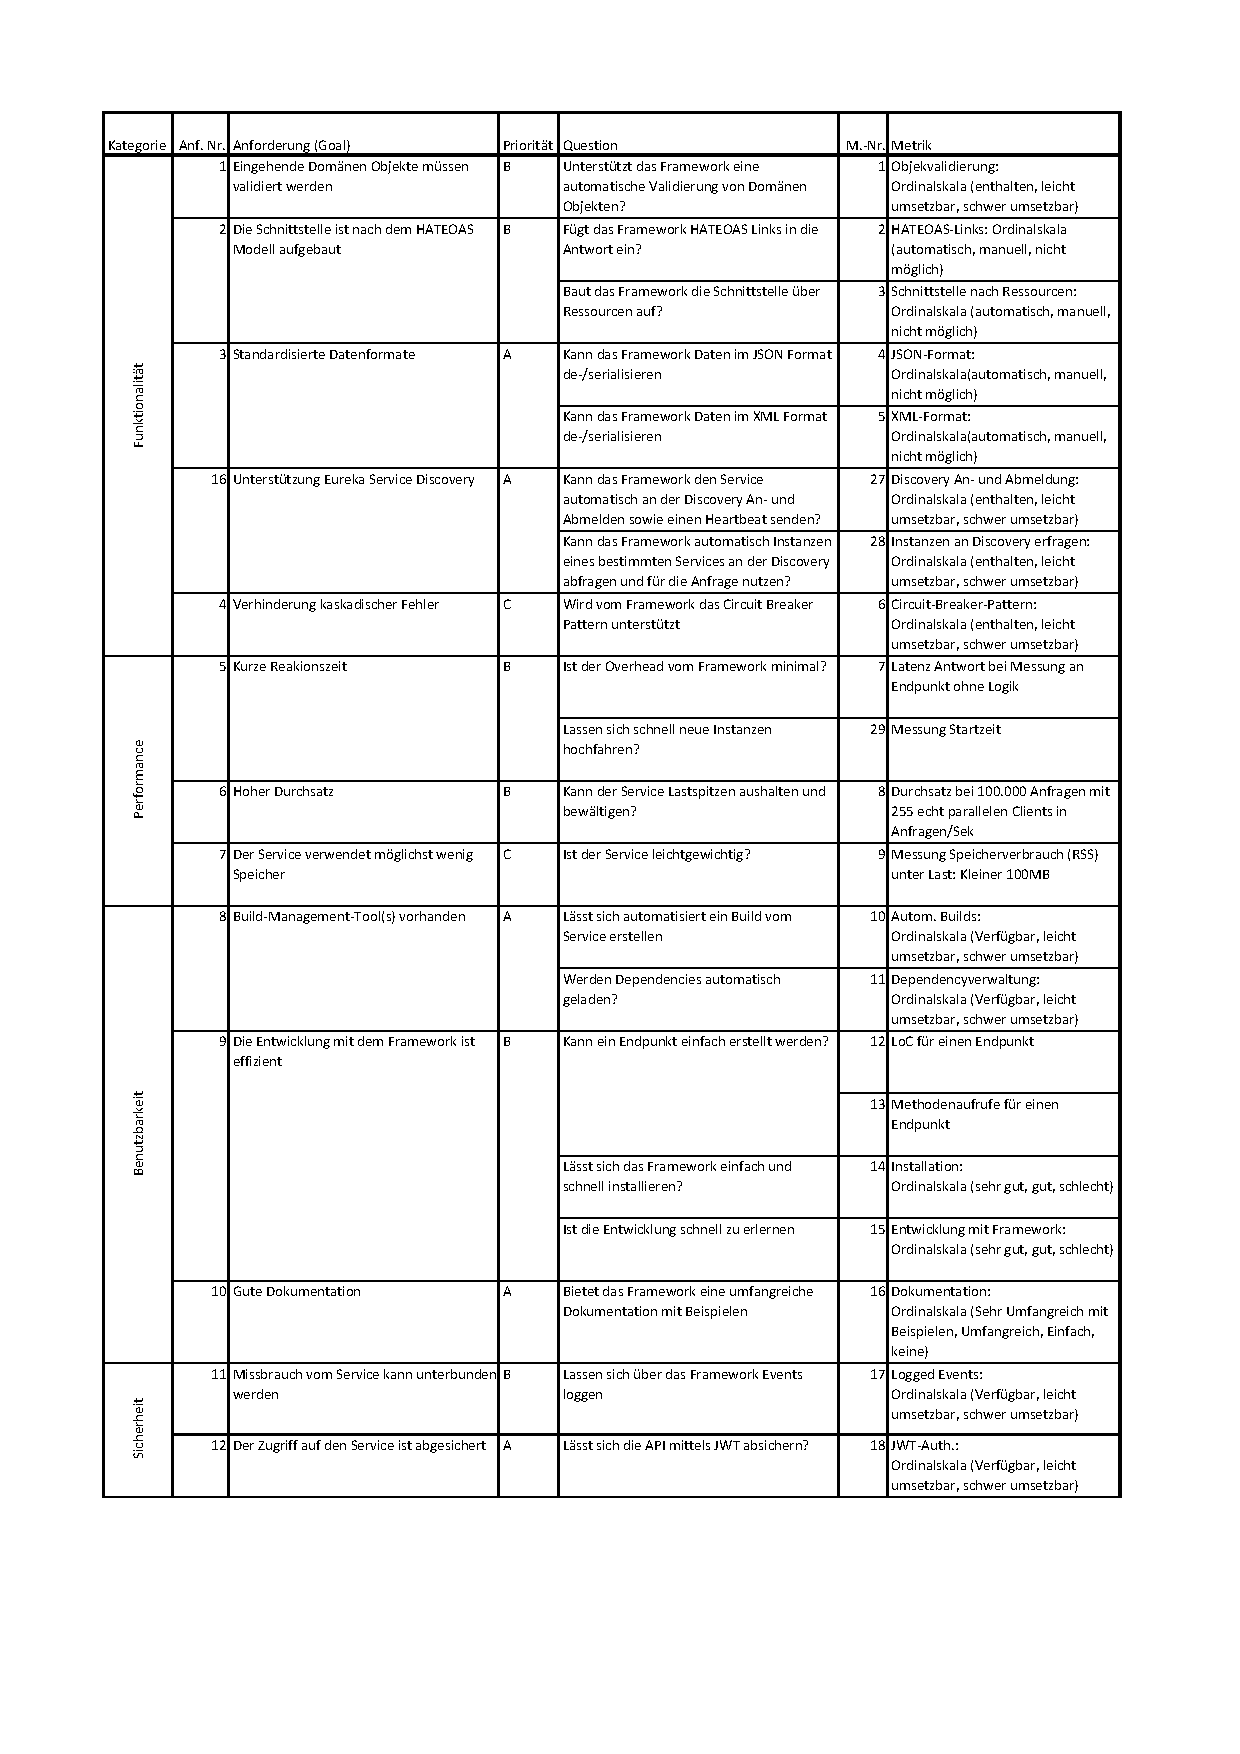
\includegraphics[width=\linewidth]{Bilder/GQM.pdf} \\	
	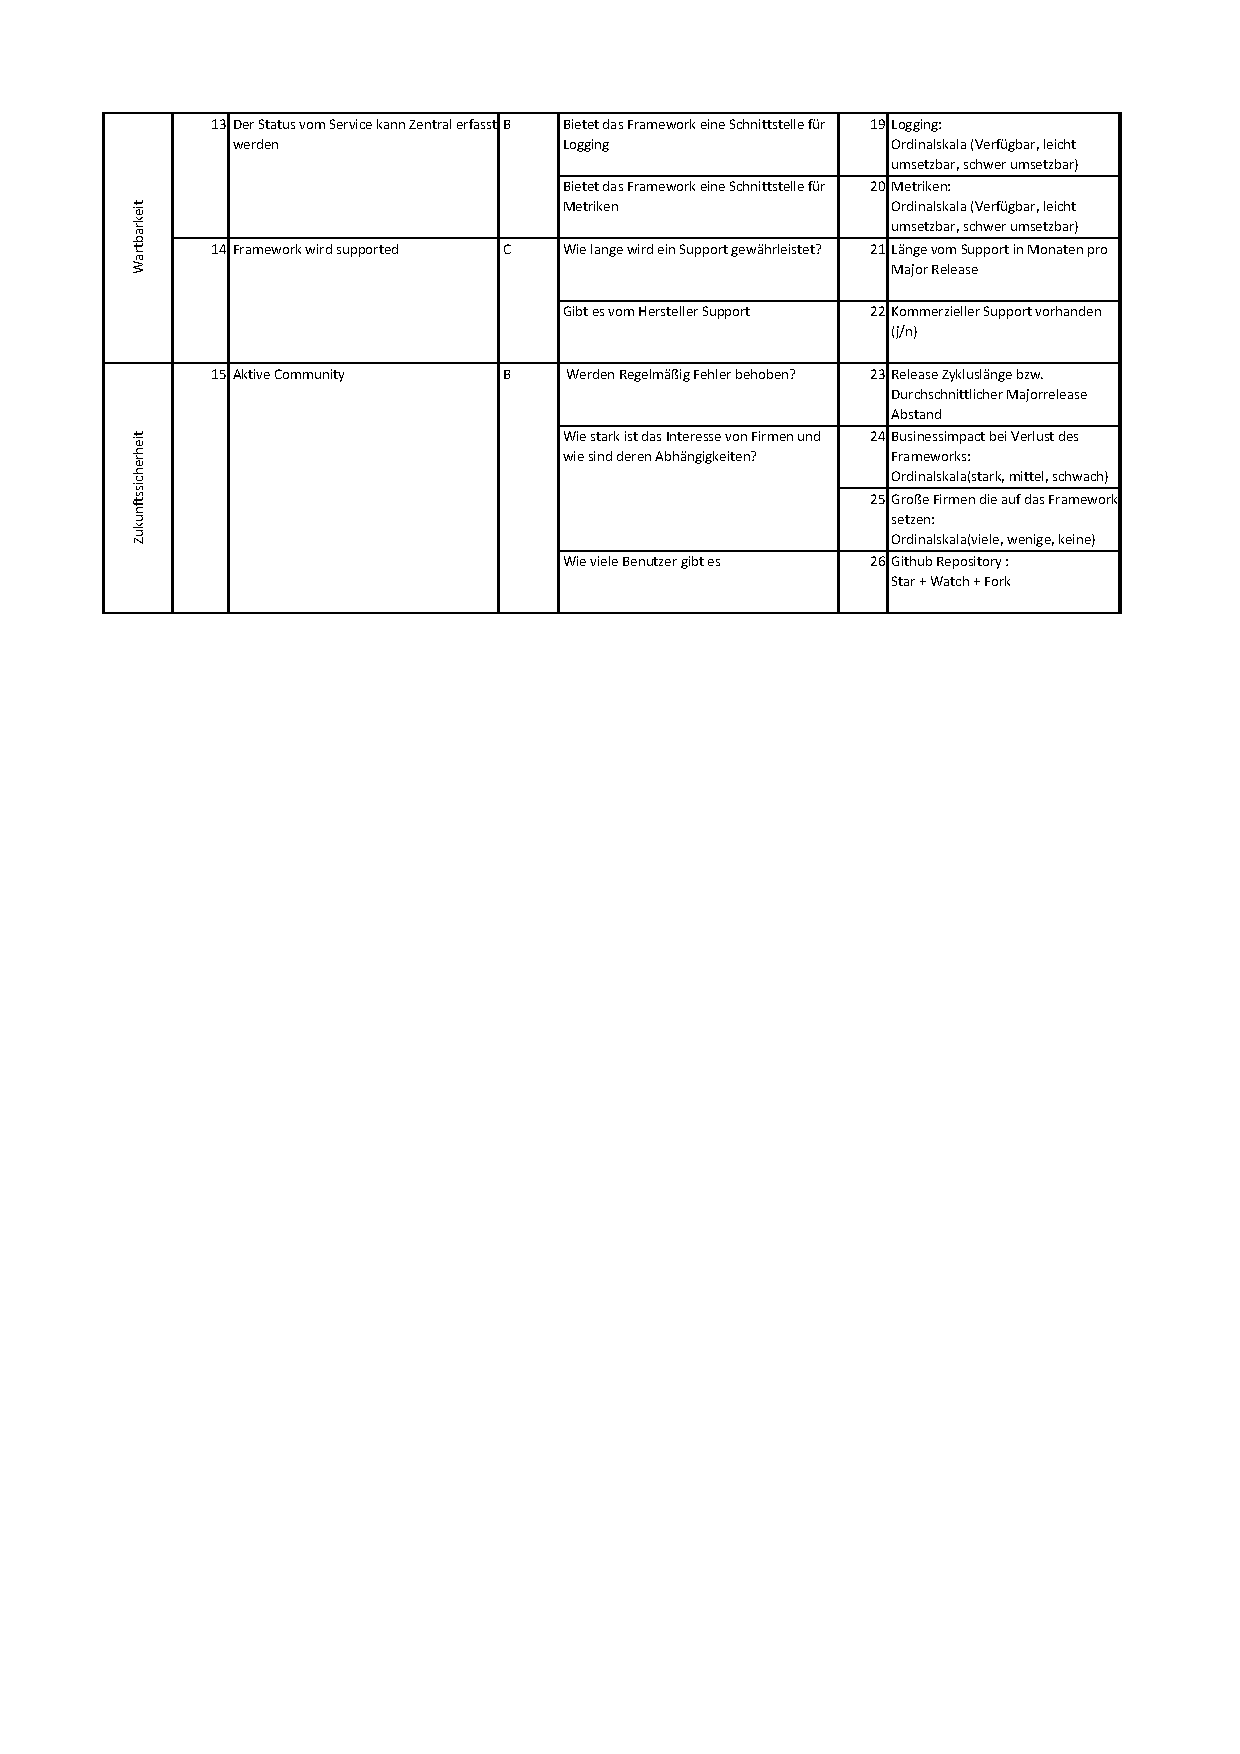
\includegraphics[width=\linewidth]{Bilder/GQM2.pdf}	\\
	\caption[Evaluation: Goal Question Metrik Tabelle]{Goal Question Metrik Ergebnis}
	\label{GQM}\\
\end{longtable}
\FloatBarrier

\subsubsection{Resümee Analysephase}
Die Basisanforderungen stellen eine gute Grundlage für die Wahl der Anforderungen da und beschleunigen somit die Analysephase. Dadurch konnte der \acl{QUT} schnell aufgebaut und priorisiert werden. Es bietet sich dabei an, dass der \ac{QUT} mit den Basisanforderungen vor dem Brainstorming für die Anforderungen vorbereitet ist und entsprechend angepasst wird.\\
Bei der Definition von Metriken fällt auf, dass viele qualitative Metriken, die Ordinalskalen, verwendet wurden. Dies lässt den Ursprung von \ac{MFEM} in der qualitativen Architekturbewertung erkennen. Aus Sicht des Autors bieten die Ordinalskalen einen guten Ansatz, um auch weiche Daten zu quantifizieren. Zusammen mit den weiteren Metriken kann das Framework so von allen Seiten betrachtet werden.\\
Wie sich der Einsatz der gefunden Metriken auswirkt, kommt aus dem den folgenden Phasen hervor.

\subsection{Evaluationsphase}

In der Evaluationsphase wird nun der Ablauf der Evaluation geplant und durchgeführt. Hierzu werden im nächsten Schritt Szenarien definiert.

\subsubsection{Evaluation definieren}

Die Evaluation wird in subjektiv und objektiv aufgeteilt. Für die subjektive Evaluation werden Szenarien definiert, die die Anforderungen bzw. Metriken untersuchen sollen.\\
\ac{MFEM} sieht hierzu die Definition eines Standard-Anwendungsfalls vor, der in mehrere Teile, den Szenarien, aufgeteilt wird. Hier wurde die Erstellung eines einfachen Daten-Service definiert, der sich mit dem Beispiel aus Kapitel \ref{Evaluation_definieren} deckt. Aus diesem Grund werden auch die Beispiel-Szenarien aus Kapitel \ref{Evaluation_definieren} übernommen und hier nur kurz zusammengefasst:

\begin{description}[leftmargin=!,labelwidth=\widthof{\bfseries Sz.3 Erweiterter Service}]
	\item[Sz.1 Installation] Installation der Sprache sowie des Frameworks und Einrichtung der Build-Tools
	\item[Sz.2 Einfacher Service] Programmierung eines einfachen "Hello World"-Services, inklusive Security
	\item[Sz.3 Erweiterter Service] Erweiterung des einfachen Services um ein Datenmodell (Aufgabenverwaltung)  
\end{description} 

Für die objektive Evaluation stehen nach \ac{MFEM} bereits Messgruppen fest. Diese umfassen die Messung an Artefakten, wie z.~B. dem Code, die Performance-Messung am lauffähigen Prototyp sowie der Recherche.\\
Um für die Messungen am laufenden Prototyp definierte Umstände zu haben, werden hier noch Anforderungsprofile benötigt. Dabei wurden folgende Profile für die Evaluation festgehalten:

\begin{table}[!h]
	\centering
	\begin{tabular}{p{1cm}p{4cm}p{2cm}p{2cm}p{4cm}}
		\textbf{Nr.} & \textbf{Typ} & \textbf{Parallele Verbindungen} & 
		\textbf{Dauer} & \textbf{Besonderheit} \\
		\hline
		1 	& Datenservice 			& 255	&	30s		& CRUD Operationen auf Datenbank  \\
		\hline
		2	& Einfacher Service		& 255 	&	30s		& Wenig rechenintensive Geschäftslogik   \\
		\hline
	\end{tabular}
	\caption[Anforderungsprofile]{Anforderungsprofile für die objektiven Evaluation am Prototyp}
	\label{AnforderungsprofileEval}
\end{table}

Insgesamt ergeben sich für den nächsten Schritt somit 6 Messgruppen, denen Metriken zugeordnet werden können.
Diese sind in Abbildung \ref{MessgruppenEval} nochmal zusammengefasst.

\image[MessgruppenEval.pdf]{MessgruppenEval}{Messgruppen für Evaluation}{Zusammenfassung aller Messgruppen für Evaluation}

\subsubsection{Metriken zuordnen}

Die Zuordnung der Metriken beginnt mit den Szenarios. Da diese zur subjektiven Evaluation gehören, werden nur weiche Daten erhoben. Im aktuellen Fall betrifft dies somit die mittels Ordinalskala erhobenen Metriken.

Da das Szenario 1 die Installation und Einrichtung übernimmt, wurden hier z.~B. Metriken der Anforderungen \enquote{Build-Tools} oder \enquote{Dependencieverwaltung} zugeordnet. Mit dem Szenario 2, dem einfachen Service, konnten die Standardformate und Security (\ac{JWT}) zugeordnet werden. Als letzte wurden dem Szenario 3, dem erweiterten Service, die Metriken für die \ac{REST}-Schnittstelle sowie Objektvalidierung zugeordnet. Zusätzlich wurden diesem Szenario, da es das Fortgeschrittenste ist, auch die Dokumentation und effiziente Programmierung zugeteilt.\\
Somit blieben am Ende des ersten Durchlaufs Metriken für Anforderungen wie z.~B. Logging, Service-Discovery und Circuit-Breaker-Pattern übrig. Aus diesem Grund mussten die Szenarios weiter verfeinert werden. Die Wahl fiel dabei auf das Szenario 2. Es sollte somit nicht nur ein "Hello World"-Service entstehen, sondern auch ein Service der bereits in der Infrastruktur funktioniert. Somit ließen sich auch die letzten Metriken zuordnen. 

Es ergibt sich somit die in Tabelle \ref{SzMetriken} gezeigte Zuordnung.  

\begin{longtable}{c}
	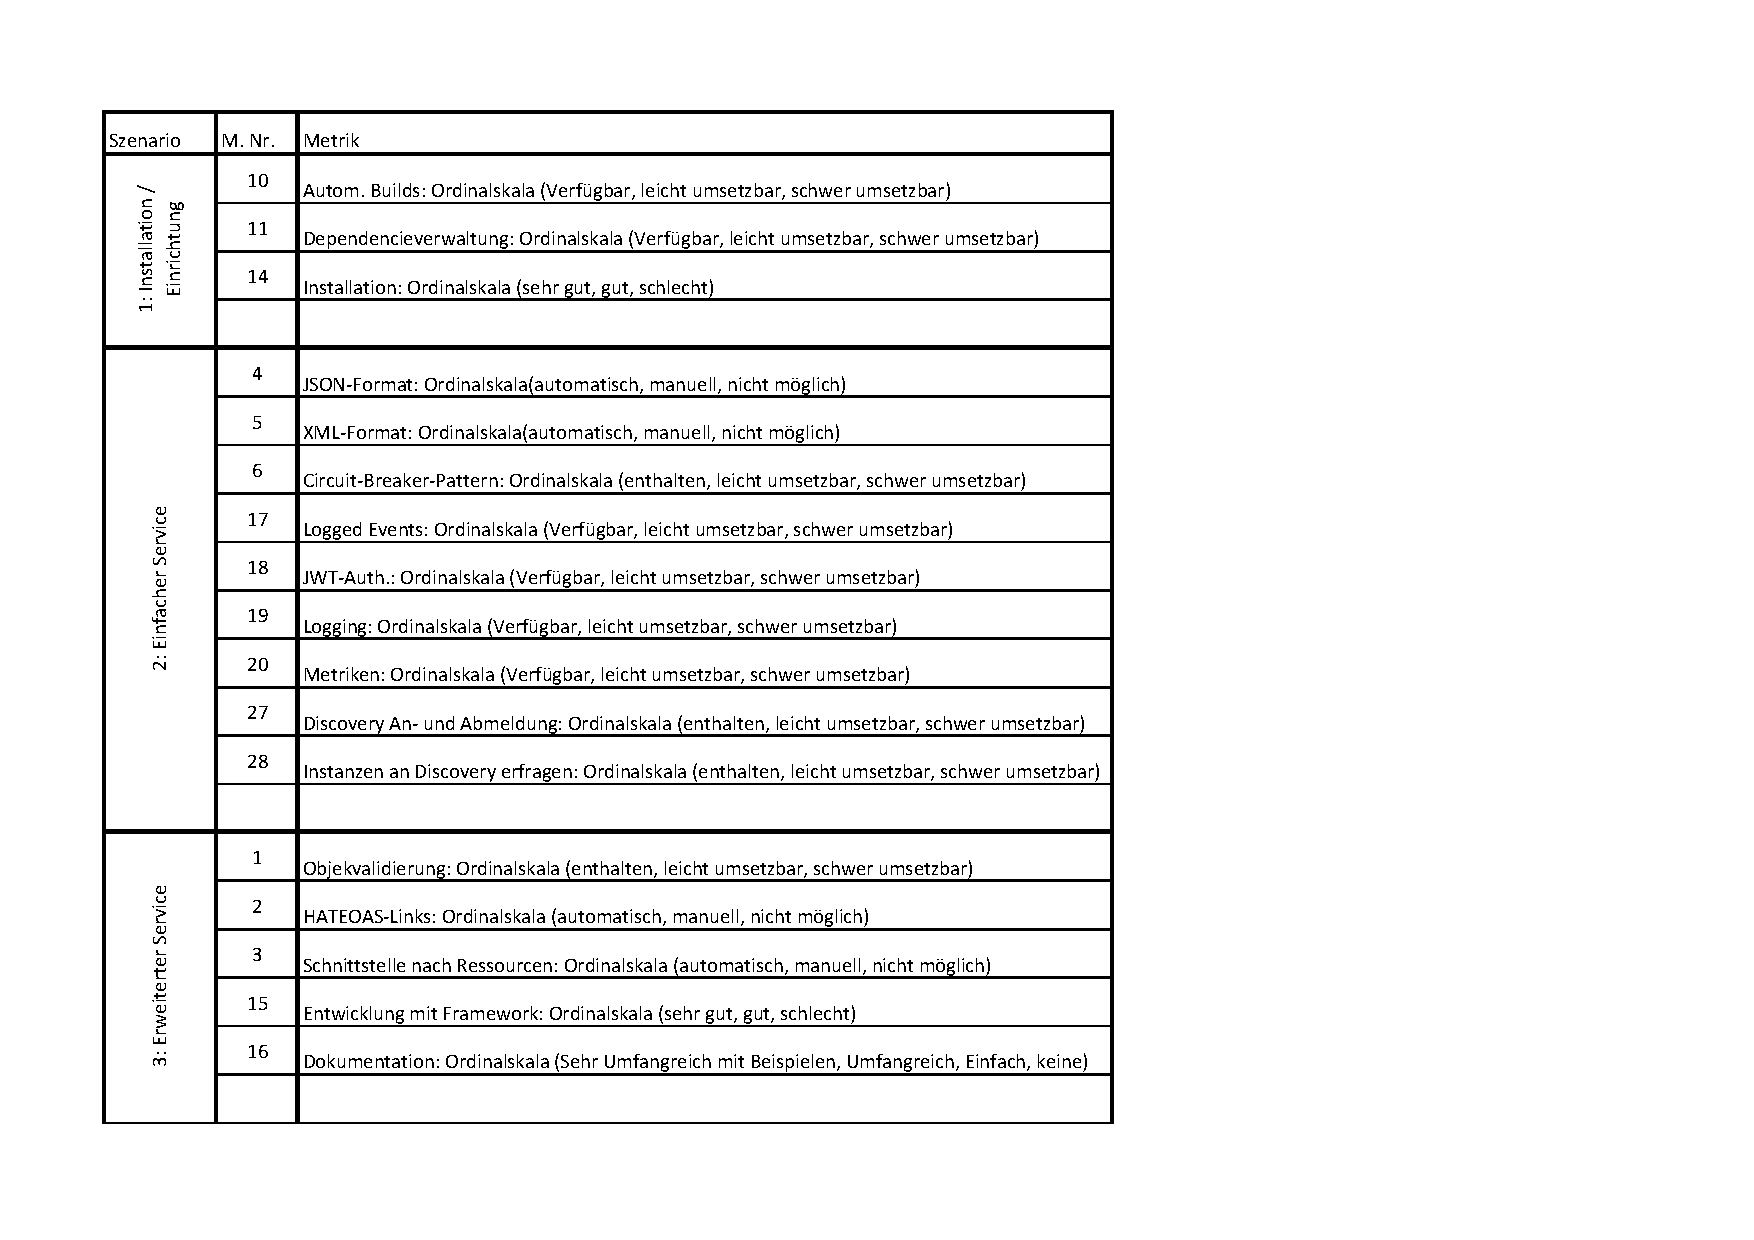
\includegraphics[width=\linewidth]{Bilder/SzMetriken.pdf} \\	
	\caption[Metriken Szenarios]{Szenarios: Zugeordnete Metriken}
	\label{SzMetriken}\\
\end{longtable}
\FloatBarrier

Da die objektiven Metriken sich nur an ihrem definierten Messpunkt erheben lassen, z.~B. kann der Durchsatz nur am lauffähigen Prototyp ermittelt werden, ließen sich diese einfach auf die 3 verbleibenden Messgruppen verteilen. 

Es ergibt sich somit die in Tabelle \ref{ObjekEvalMetriken} gezeigte Zuordnung. 

\begin{longtable}{c}
	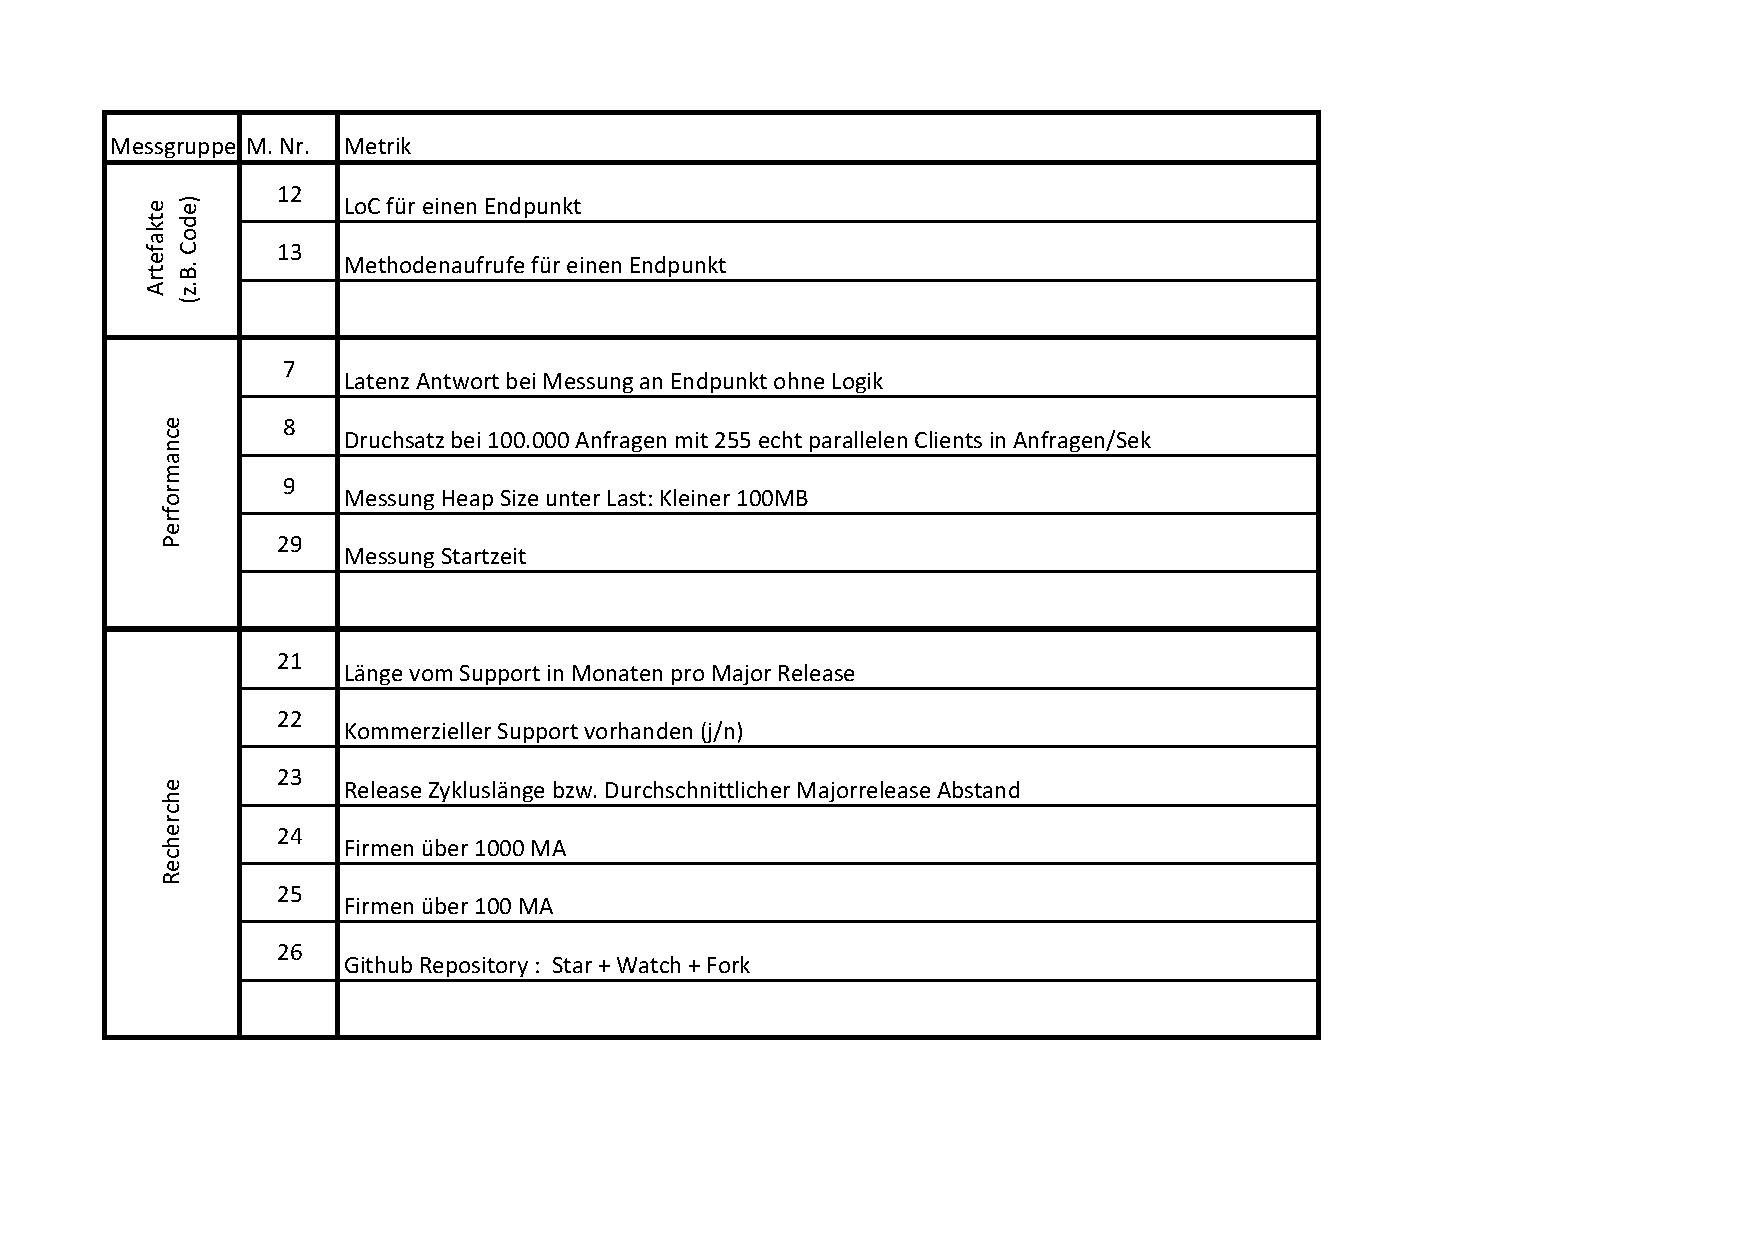
\includegraphics[width=\linewidth]{Bilder/ObjekEvalMetriken.pdf} \\	
	\caption[Metriken Objektive Evaluation]{Objektive Evaluation: Zugeordnete Metriken}
	\label{ObjekEvalMetriken}\\
\end{longtable}
\FloatBarrier

Da nun festgelegt ist, an welchem Punkt welche Daten erhoben werden, kann die Evaluation der Kandidaten durchgeführt werden.

\subsubsection{Evaluation durchführen: Spring Boot}

An dieser Stelle werden die Szenarien und Messungen an Spring Boot vorgenommen. Da es bei der Evaluation von \ac{MFEM} weniger um die konkrete Implementierung\footnote{
	Die gesamte Implementierung findet sich auf einem Github Repository mit der URL:\url{https://github.com/darenegade/SimpleSpringService}
} 
 geht, wird die Durchführung der einzelnen Messgruppen nur kurz beschrieben. Dabei werden markante Punkte hervorgehoben, sodass die Ergebnisse nachvollziehbar bleiben. 

\newparagraph{Szenario 1: Installation}
Mit Spring Boot wird Java als Programmiersprache benötigt. Die nötigen Installationsdateien lassen sich für jedes Betriebssystem bei Oracle\footnote{\url{http://www.oracle.com/technetwork/java}} beziehen.\\
Als Buildmanagement-Tools haben sich Gradle\footnote{\url{https://gradle.org}}  und Maven\footnote{\url{https://maven.apache.org}} etabliert. Beide sind für die Verwendung mit Spring gut geeignet. Und da keines augenscheinlich einen Vorzug aufweist, wurde Maven gewählt. Die Installation ist sehr einfach und es werden keine Vorkenntnisse benötigt. So konnten alle Metriken mit den bestmöglichen Werten bewertet werden.

\begin{longtable}{c}
	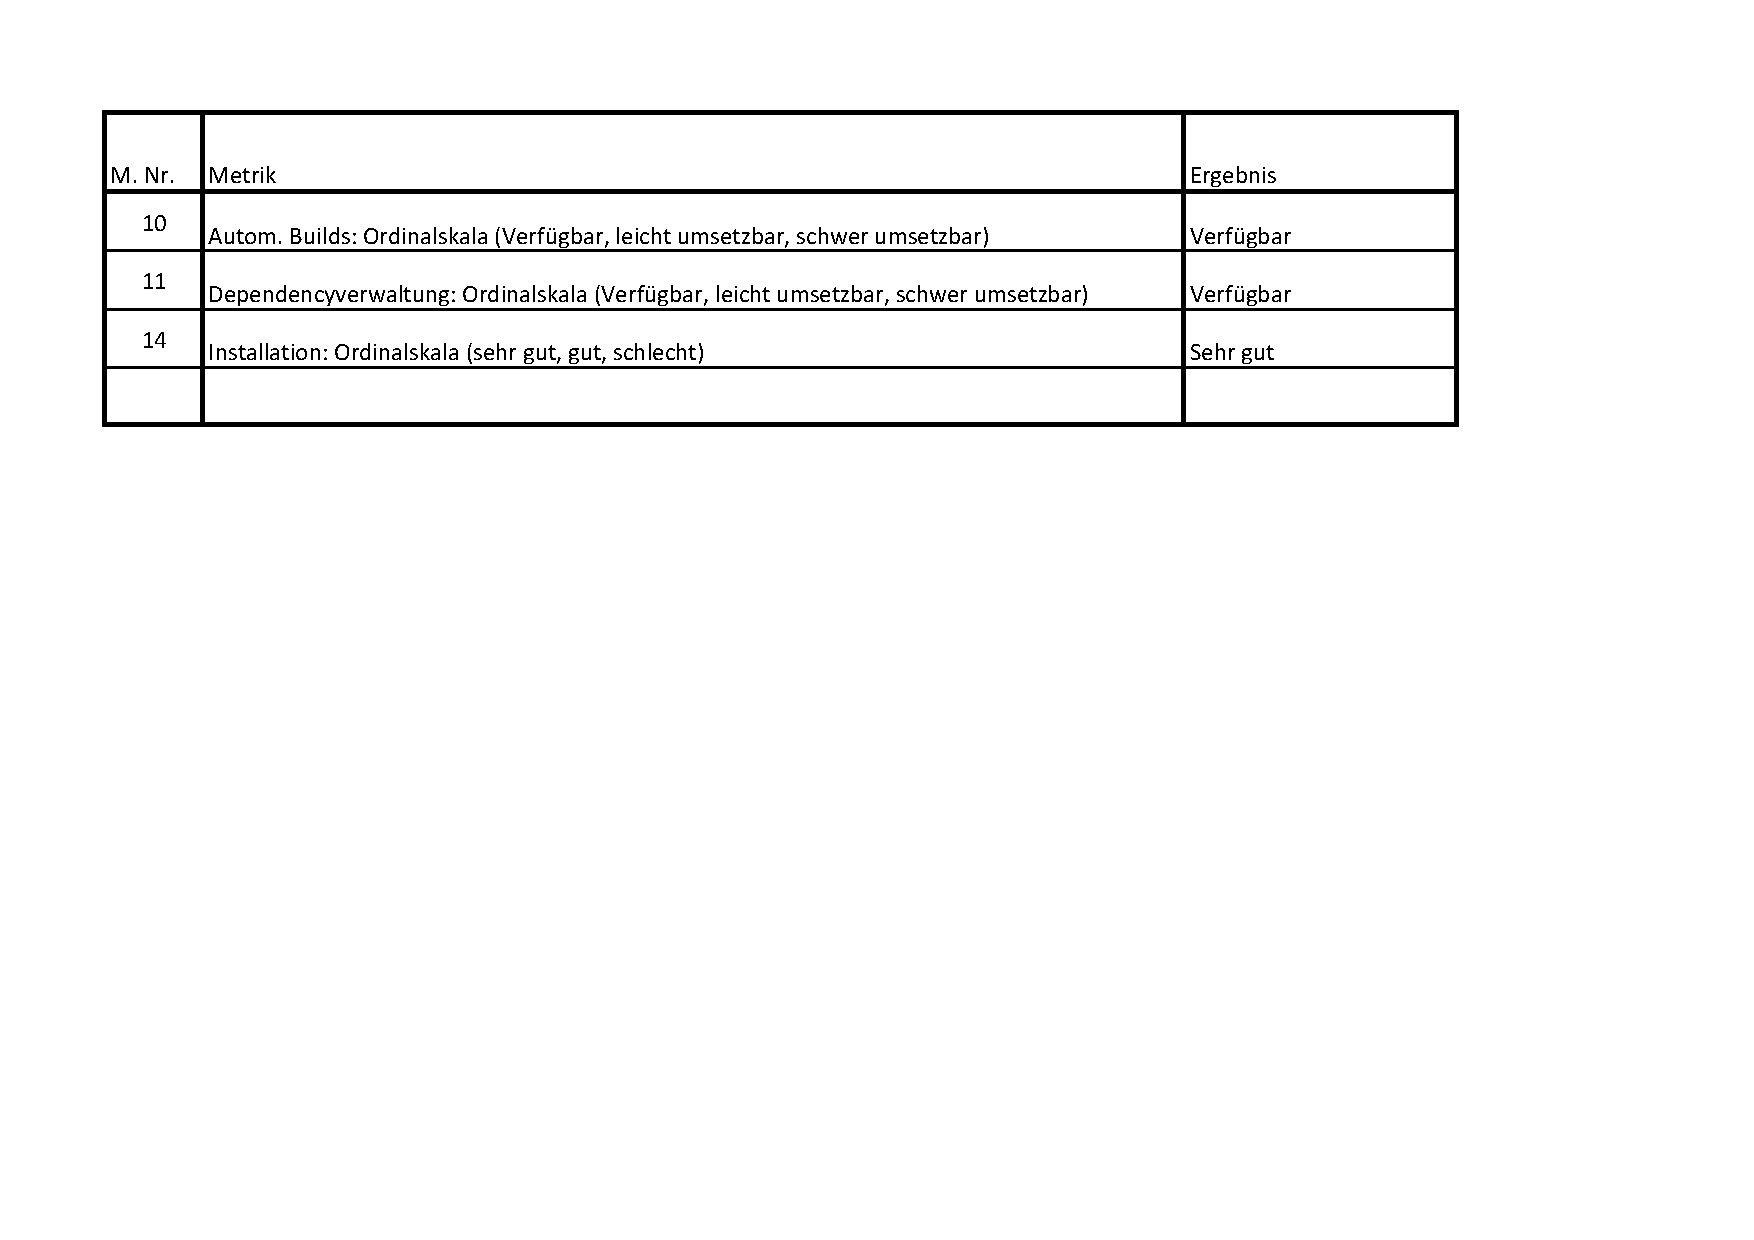
\includegraphics[width=\linewidth]{Bilder/Sz1ErgebnisSpring.pdf} \\	
	\caption[Szenario 1 Ergebnis Spring]{Ergebnis von Szenario 1 für Spring}
	\label{Sz1ErgebnisSpring}\\
\end{longtable}
\FloatBarrier

\newparagraph{Szenario 2: Einfacher Service}
Für die Erstellung eines neuen Projektes bietet Spring einen Initialisierungsservice\footnote{\url{http://start.spring.io}} an. Dieser lässt einen die nötigen Spring Module auswählen und das Projekt vorkonfigurieren. Als Ergebnis erhält man ein vollständig konfiguriertes Maven Projekt.
Dies macht den Einstieg sehr unkompliziert.

Auch die Implementierung eines "Hello-World"-Service ist mit Spring denkbar einfach. Das Listing \ref{SpringHello} zeigt was hierfür nötig ist. Daran sieht man sehr gut, dass die Einstiegshürde sehr gering ist. 
Mit \lstinline|@SpringBootApplication| werden die Standard-Spring\-konfigurationen aktiviert. So lässt sich anschließend über \lstinline|@RestController| und \lstinline|@PostMapping| der "Hello-World"-Endpunkt erstellen.
Mehr Konfiguration ist dabei nicht nötig, da Spring über die automatische Konfiguration die Parameter sowie den Rückgabewert der Methode erkennt und damit den Endpunkt anlegt. Auch die De- und Serialisierung in die Standardformate erfolgt automatisch und muss nicht manuell erstellt werden. Somit konnten diese Anforderungen mit \enquote{automatisch} bewertet werden. 

\begin{minipage}{\linewidth}
	\begin{lstlisting}[caption={"Hello-Word" in Spring},label=SpringHello,language=JAVA] 
		@SpringBootApplication
		@RestController
		@EnableEurekaClient
		public class Application {
		
			public static void main(String[] args) {
				SpringApplication.run(Application.class, args);
			}
			
			@PostMapping("/hello_service")
			public String helloService(@RequestBody Name name){
				return "Hello " + name.getName();
			}
		}
	\end{lstlisting}
\end{minipage}

Ähnlich mühelos gestaltet sich die Einrichtung der Service-Discovery Unterstützung. Mit der zusätzlichen Annotation \lstinline|@EnableEurekaClient| und einem Eintrag der Discovery-URL in der Datei \lstinline|application.properties| ist der Service für die Discovery konfiguriert. Die zugehörige Anforderung konnte somit bestmöglich bewertet werden. \\
Diese Kombination von Annotationen und einfachen Konfigurationen ist typisch für Spring Boot und konnte auf sämtliche weiteren Anforderungen angewendet werden. Das Ergebnis in Tabelle \ref{Sz2ErgebnisSpring} ist dementsprechend positiv.

\begin{longtable}{c}
	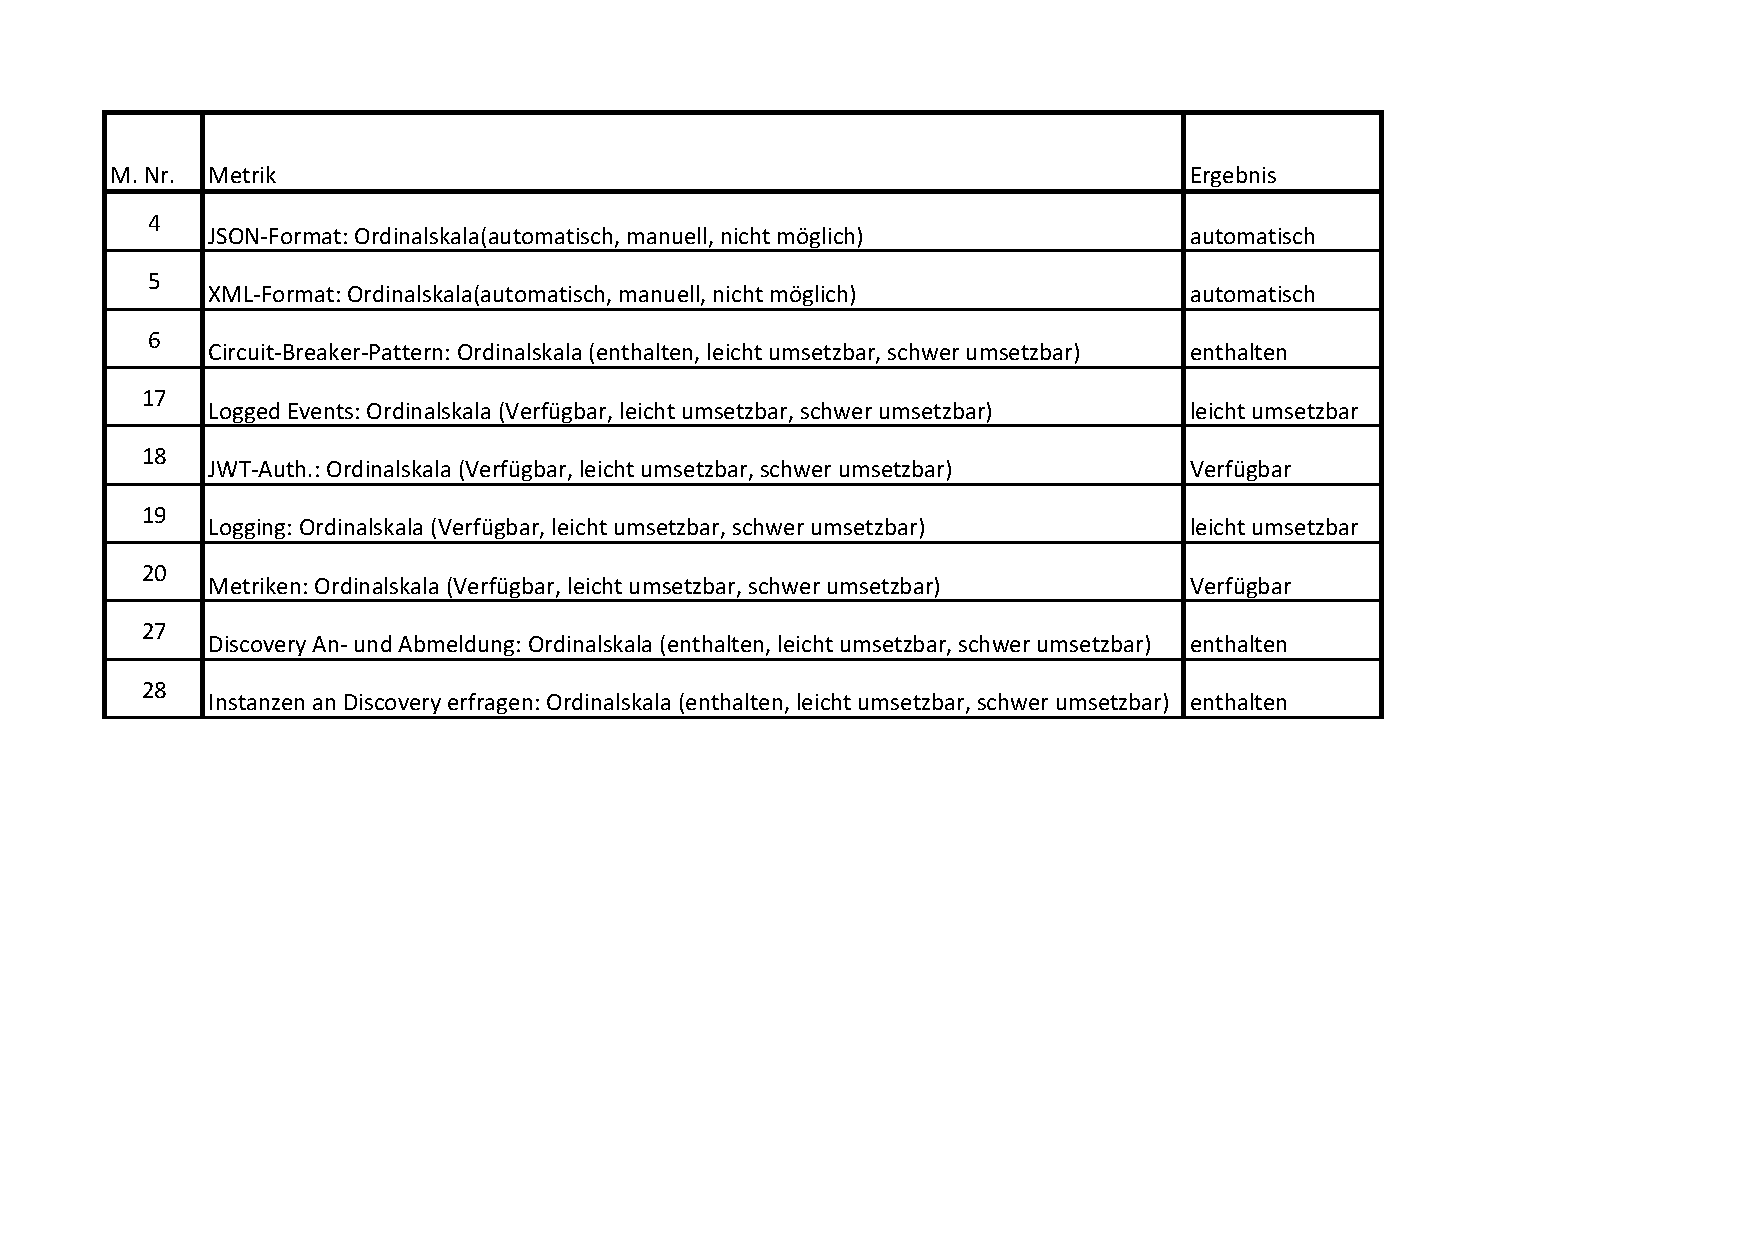
\includegraphics[width=\linewidth]{Bilder/Sz2ErgebnisSpring.pdf} \\	
	\caption[Szenario 2 Ergebnis Spring]{Ergebnis von Szenario 2 für Spring}
	\label{Sz2ErgebnisSpring}\\
\end{longtable}
\FloatBarrier

\newparagraph{Szenario 3: Erweiterter Service}
Das Szenario 3 sieht vor das Datenmodell für die Aufgabenverwaltung (Abbildung \ref{Datenmodell}) zu implementieren und über eine \ac{REST}-Schnittstelle nach außen anzubieten. Das Datenmodell wird dabei über die \ac{JPA} für Spring aufgebaut und die Konfiguration besteht somit auch aus Annotationen. Listing \ref{Department} zeigt dies als Beispiel für die Entität \enquote{Department}.

\begin{minipage}{\linewidth}
	\begin{lstlisting}[caption={Umsetzung der Entität \enquote{Department} mittels JPA},label=Department,language=JAVA] 
	@Entity
	public class Department extends BaseEntity{
	String name;
	
	@OneToOne
	@NotNull
	Employee head;
	
	@OneToMany
	Set<Employee> employees;
	
	//... Getter + Setter 
	}
	\end{lstlisting}
\end{minipage}

Die Besonderheit von Spring ist nun, dass mittels Spring-Data-Rest und dem in Listing \ref{DepRepo} gezeigten Code, die komplette \ac{REST}-Schnittstelle fertig konfiguriert ist. Das Repository-Interface muss lediglich als solches mit der Annotation \lstinline|@RepositoryRestResource| gekennzeichnet und von \lstinline|CrudRepository<T, ID>| abgeleitet werden, sodass Spring die Schnittstelle aufbauen kann. Diese ist vollständig nach Ressoucen aufgebaut und integriert in die Antworten automatisch \acs{HATEOAS} Links.

\begin{minipage}{\linewidth}
	\begin{lstlisting}[caption={Erstellung der REST-Schnittstelle für das \enquote{Department} über ein Interface},label=DepRepo,language=JAVA] 
	@RepositoryRestResource
	public interface DepartmentRepository extends 
									CrudRepository<Department, UUID> { 
	}
	\end{lstlisting}
\end{minipage}

Die Entwicklung eines Datenservice könnte somit kaum effizienter sein. Die automatische Konfiguration lässt sich auch anpassen. Hierzu bietet die Dokumentation detaillierte Beschreibungen und Code-Beispiele.\\
Somit konnte auch im 3. Szenario Spring sehr gut bewertet werden. Das Ergebnis ist in Tabelle \ref{Sz3ErgebnisSpring} zu sehen.

\begin{longtable}{c}
	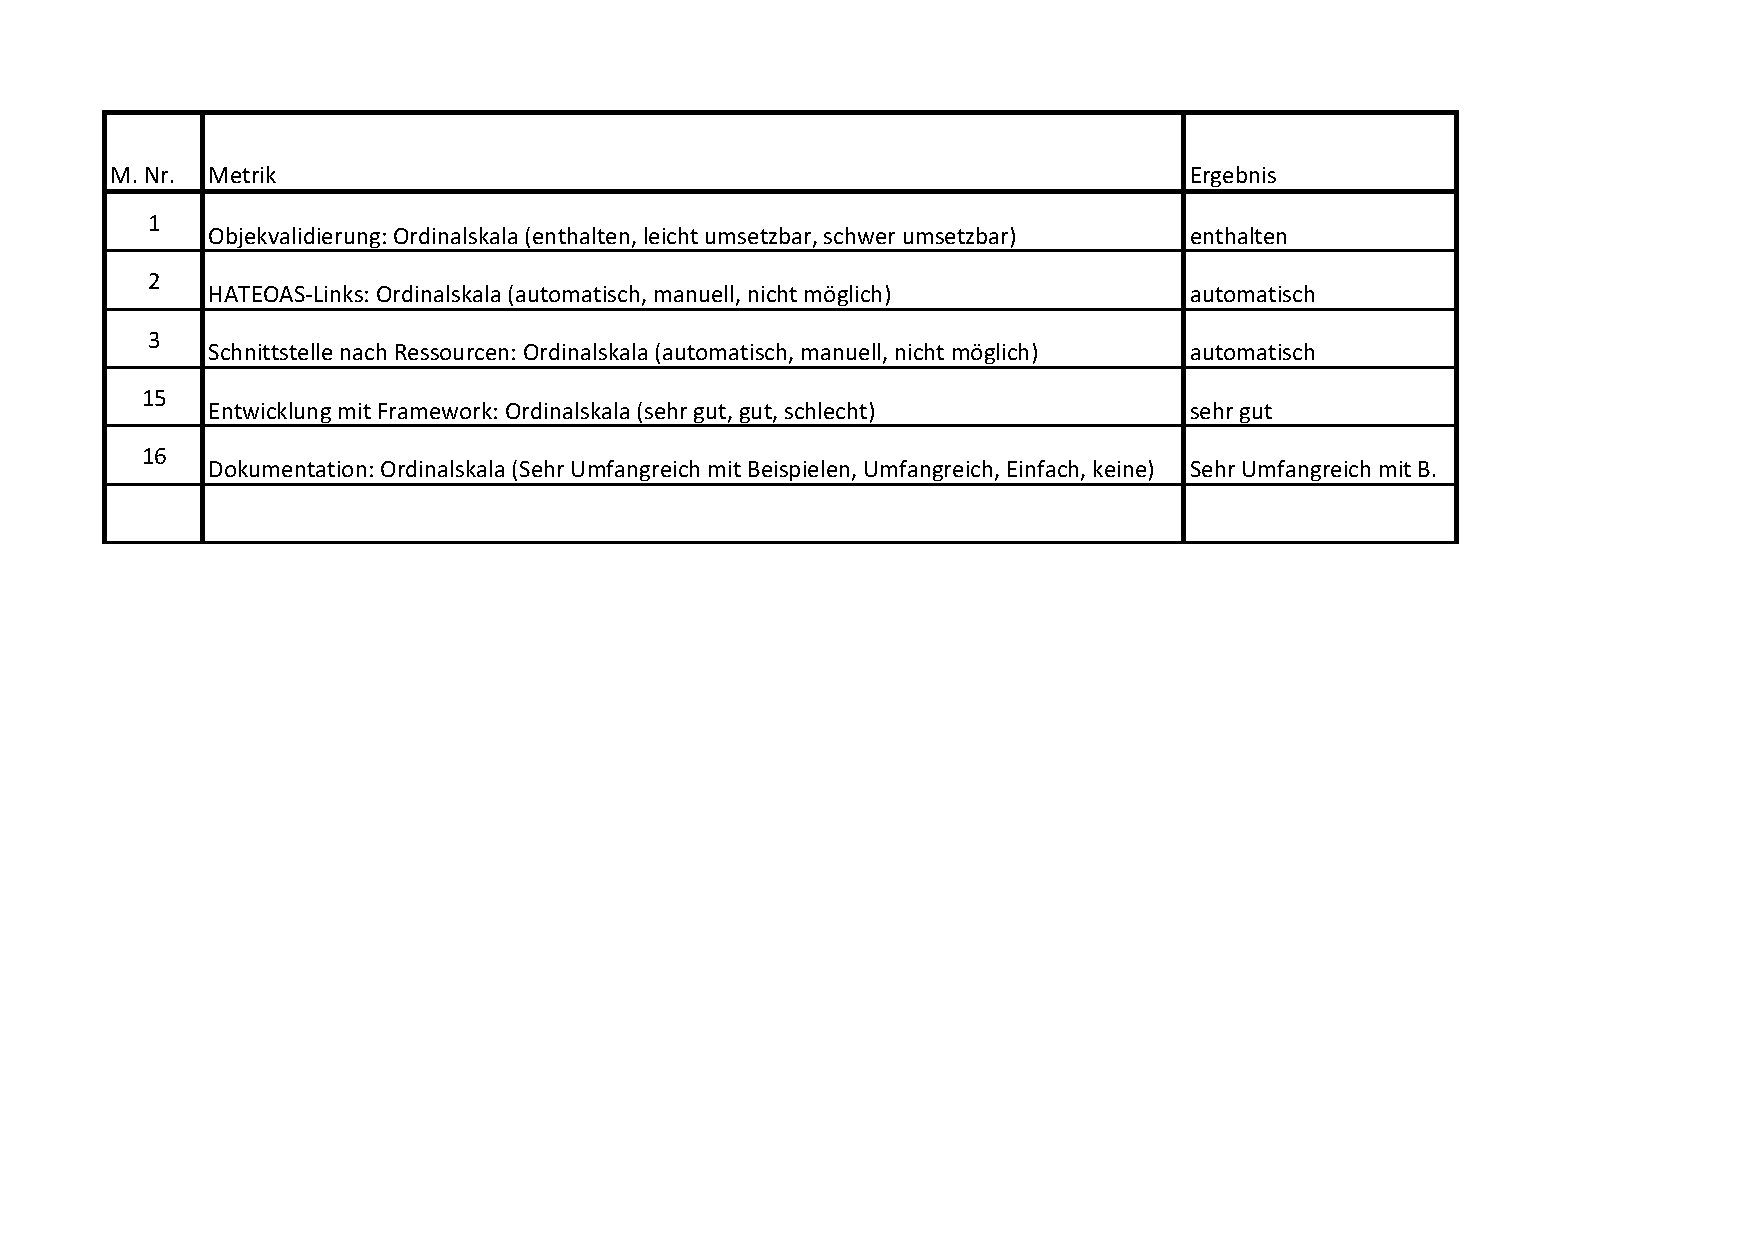
\includegraphics[width=\linewidth]{Bilder/Sz3ErgebnisSpring.pdf} \\	
	\caption[Szenario 3 Ergebnis Spring]{Ergebnis von Szenario 3 für Spring}
	\label{Sz3ErgebnisSpring}\\
\end{longtable}
\FloatBarrier

\newparagraph{Quantitative Evaluation}
Der aus dem 3. Szenario entstandene Prototyp kann nun für die Erhebung der harten Daten herangezogen werden. So wurden die \ac{LOC} und Methodenaufrufe für einen Endpunkt gemessen. Diese fallen, wie in Listing \ref{SpringHello} gezeigt, sehr gering aus. So bleibt die Codebasis auch bei vielen Endpunkten schlank und gut wartbar.\\
Des Weiteren wurden am lauffähigen Prototyp Performance Messungen durchgeführt. Hierzu wurde das Anforderungsprofil 2 aus der Tabelle \ref{AnforderungsprofileEval} auf den Prototyp angewendet und die entsprechenden Metriken, wie z.~B. Latenz, Durchsatz und Speicherverbrauch unter Last, gemessen\footnote{Für die Performance Messung wurde das Tool JMeter(\url{http://jmeter.apache.org}) eingesetzt und auf einem Laptop mit i7 2,3GHz Prozessor und 16GB DDR3 RAM durchgeführt.}. Die Anwendung des Anforderungsprofils 1 aus der Tabelle \ref{AnforderungsprofileEval} wurde für die Bestimmung der Metriken nicht benötigt und daher nicht weiter beachtet.

Die Recherche hat den Erwartungen entsprochen. Da Spring ein sehr etabliertes Framework ist, ist auch die Community sehr aktiv. Es werden regelmäßig Fehler behoben und neue Major-Releases veröffentlicht. Dies spiegelt auch die Akzeptanz bei großen Firmen wider. So setzen nach der offiziellen Webseite von Pivotal\footnote{\url{https://pivotal.io}}, der Organisation hinter dem Spring Framework, die 7 größten Banken oder die 9 größten Automanufakturen das Framework produktiv ein.

Die Ergebnisse der quantitativen Evaluation sind in der Tabelle \ref{QuantErgebnisSpring} festgehalten. Mit diesem Schritt wurde die Evaluation von dem Spring Framework beendet.  

\begin{longtable}{c}
	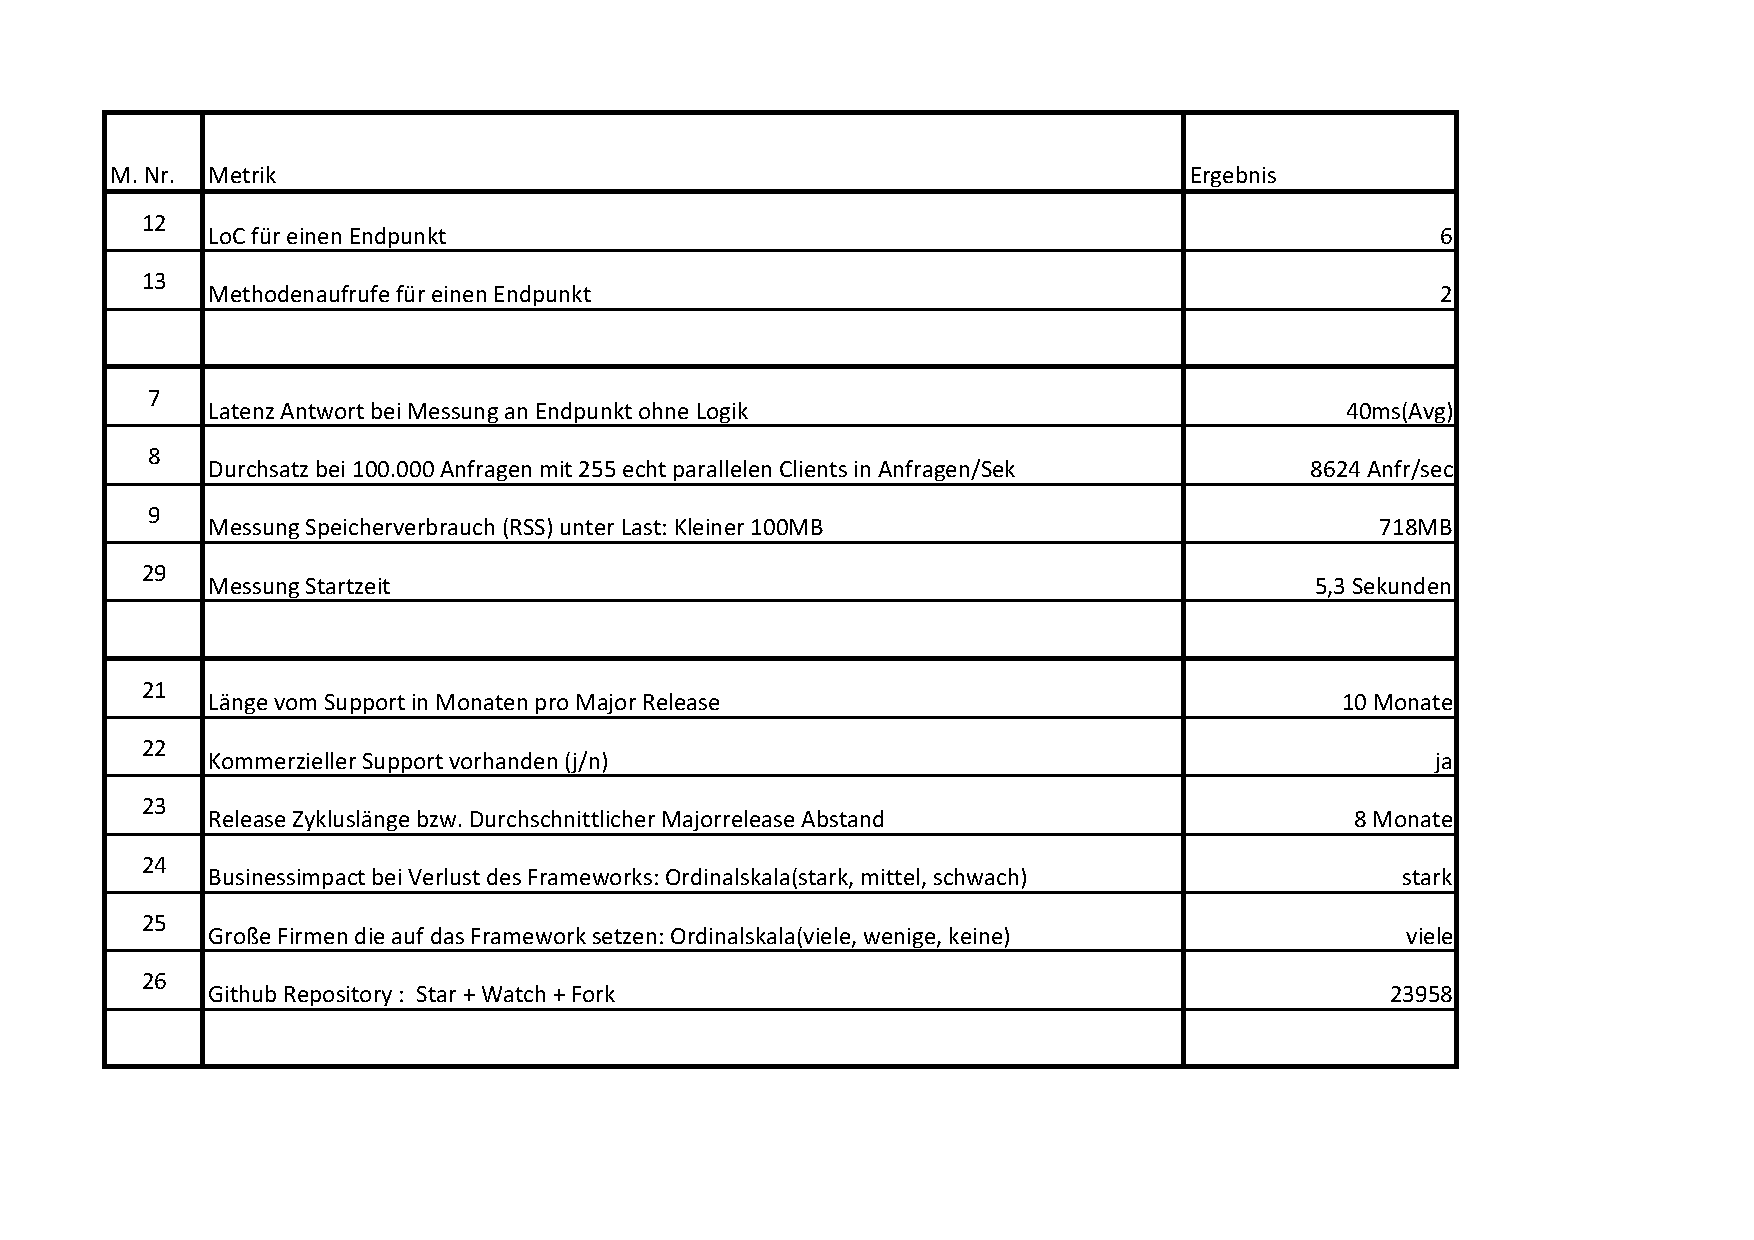
\includegraphics[width=\linewidth]{Bilder/ObjekEvalErgebnisSpring.pdf} \\	
	\caption[Quantitative Evaluation Ergebnis Spring]{Ergebnis der quantitativen Evaluation von Spring}
	\label{QuantErgebnisSpring}\\
\end{longtable}
\FloatBarrier

\subsubsection{Evaluation durchführen: Go-Kit}
Der zweite Kandidat für die Evaluation ist Go-Kit. Auch hier wird nicht auf die komplette Implementierung\footnote{
	Die gesamte Implementierung findet sich auf einem Github Repository mit der URL:\url{https://github.com/darenegade/SimpleGoKitService}
} 
eingegangen, sondern nur markante Punkte hervorgehoben. Dabei beginnt die Evaluation mit dem 1. Szenario.

\newparagraph{Szenario 1: Installation}
Go-Kit wird, wie der Name vermuten lässt, mit Go entwickelt. Daher ist die Installation von Go der erste Schritt. Hierzu lassen sich die Installationsdateien von der Webseite \url{golang.org} herunterladen und installieren.\\
Damit sind auch die essentiellen Tools für das Buildmanagement installiert. Diese sind z.~B. \lstinline|go get| für das Auflösen und Herunterladen von Abhängigkeiten (Dependencies) sowie \lstinline|go test| für das Ausführen von Unit-Tests.\\
Diese Befehle ersetzen aber kein vollständiges Buildmanagement-Tool, welches den kompletten Prozess steuert und die richtigen Abhängigkeiten auflöst\cite{GoDep2016}. So ist es notwendig den kompletten Prozess mittels Skript zu steuern und dabei Paketmanagement-Tools, wie Glide\footnote{\url{https://github.com/Masterminds/glide}}, zu nutzen.

Aus diesem Grund gab es für die Evaluation Abzüge bezüglich der Build-Tools. Die vollständige Bewertung ist in Tabelle \ref{Sz1ErgebnisGokit} festgehalten.

\begin{longtable}{c}
	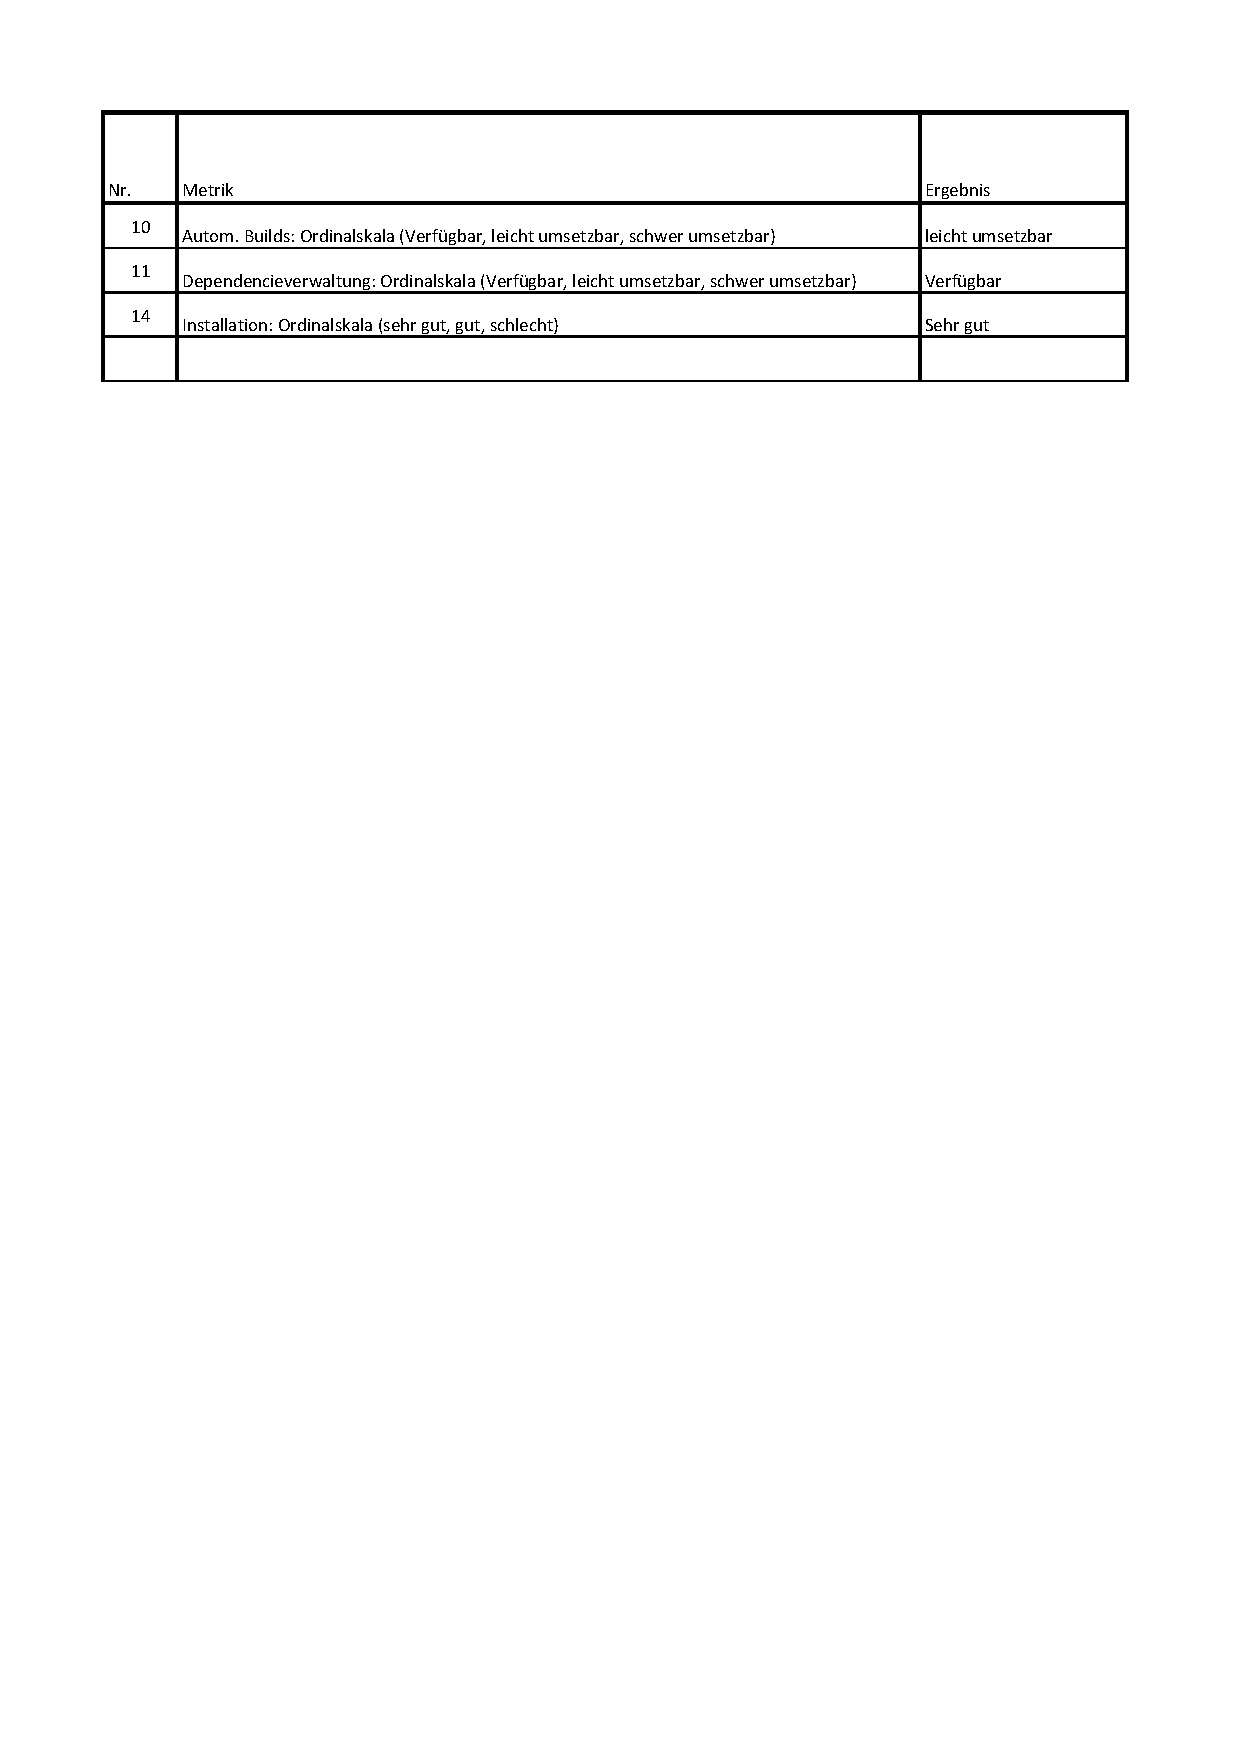
\includegraphics[width=\linewidth]{Bilder/Sz1ErgebnisGokit.pdf} \\	
	\caption[Szenario 1 Ergebnis GoKit]{Ergebnis von Szenario 1 für GoKIt}
	\label{Sz1ErgebnisGokit}\\
\end{longtable}
\FloatBarrier

\newparagraph{Szenario 2: Einfacher Service}
Im 2. Szenario wird ein einfacher "Hello World"-Service implementiert. Hierzu muss ein neues Projekt angelegt werden, welches im Workspace von Go, dem GoPath, erfolgen muss. Dabei ist das \lstinline|main.go| File der Einstiegspunkt einer jeden Go Applikation.\\
Die Implementierung des einfachen "Hello-Word"-Endpunktes ist in Listing \ref{HelloGo} dargestellt.

\begin{lstlisting}[caption={"Hello-Word" in Go-Kit},label=HelloGo,language=Golang] 
	func main() {
		logger := LOG.NewLogfmtLogger(os.Stdout)
		ctx := context.Background()
		svc := helloWorldService{}
		
		var helloWorldEndpoint endpoint.Endpoint
		helloWorldEndpoint = makeHelloWorldEndpoint(svc)
		
		helloWorldHandler := httptransport.NewServer(
			ctx, helloWorldEndpoint, 
			decodeHelloWorldRequest, encodeResponse,
			httptransport.ServerErrorLogger(logger),
		)
		
		http.Handle("/hello_service", helloWorldHandler)
		log.Fatal(http.ListenAndServe(":8080", nil))
	}
	
	type HelloWorldService interface {
		helloService(string) (string, error)
	}
	
	type helloWorldService struct{}
	
	func (helloWorldService) helloService(name string) (string, error) {
		return "Hello " + name, nil
	}
\end{lstlisting}

Dies zeigt sehr deutlich, dass die Erstellung eines Endpunktes relativ komplex ist. Es erfordert mehrere Konfigurationsschritte und muss vollständig manuell erfolgen, wobei der Ausschnitt nur ein Teil der gesamt nötigen Implementierung darstellt.\\
Auch ist die Verbindung zur Service Discovery an der Stelle noch nicht eingebaut. Go-Kit bietet für Eureka keine Unterstützung, sodass diese komplett eigenständig entwickelt werden muss. Da diese Anforderung mit \enquote{A} bewertet wurde und auch weitere Metriken ein mittelmäßiges Ergebnis aufweisen, könnte an dieser Stelle bereits über ein Abbruch der Evaluation diskutiert werden.\\
Im Sinne der Evaluation von \ac{MFEM} wurde entschieden, die Durchführung nicht abzubrechen. Das dabei entstanden Ergebnis ist in Tabelle \ref{Sz2ErgebnisGokit} zusammengefasst.

\begin{longtable}{c}
	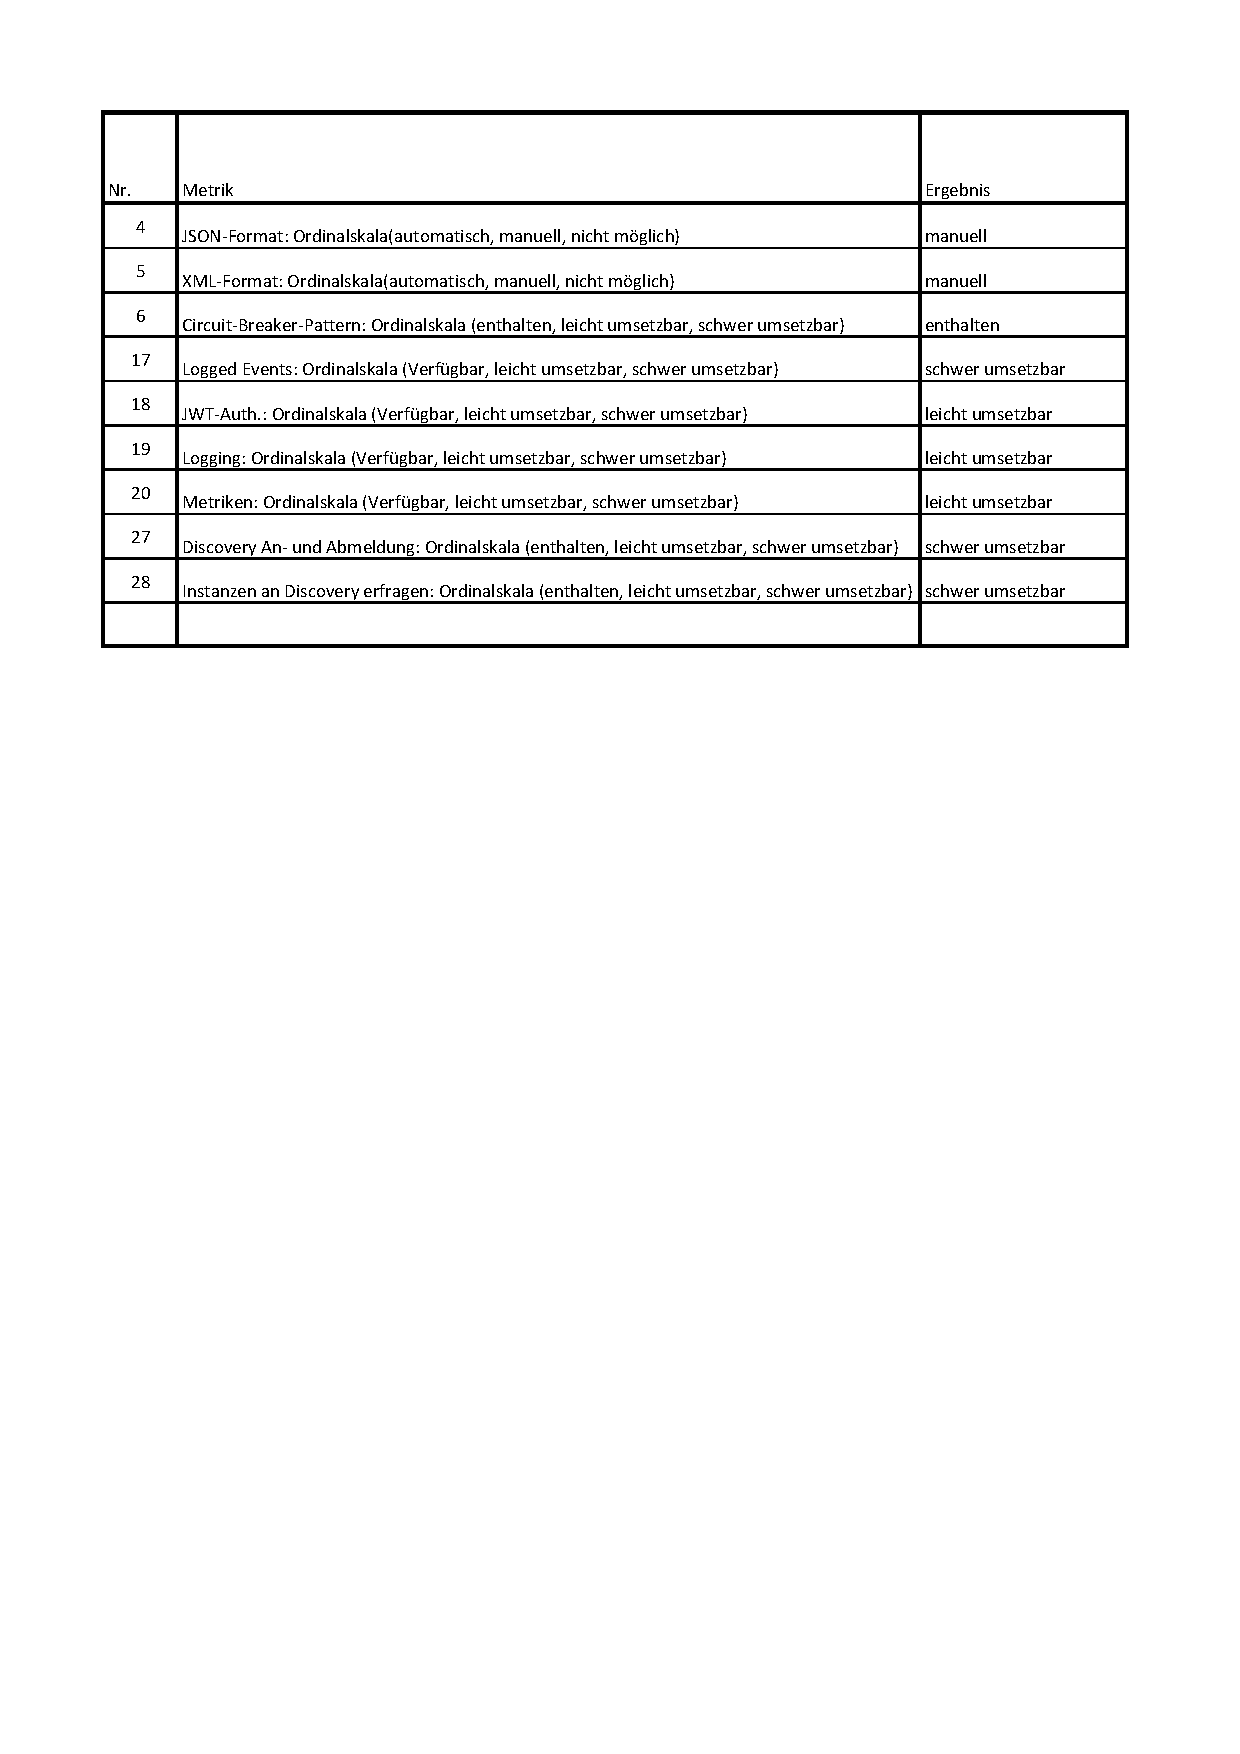
\includegraphics[width=\linewidth]{Bilder/Sz2ErgebnisGokit.pdf} \\	
	\caption[Szenario 2 Ergebnis GoKit]{Ergebnis von Szenario 2 für GoKIt}
	\label{Sz2ErgebnisGokit}\\
\end{longtable}
\FloatBarrier    

\newparagraph{Szenario 3: Erweiterter Service}
Auch beim erweiterten Service stößt man mit Go-Kit schnell an die Grenzen. Es bietet selber keine Unterstützung für eine Verbindung zu einer MySQL Datenbank. Um dies zu ermöglichen, wurde die Gorm\footnote{\url{http://jinzhu.me/gorm/}} Bibliothek mit aufgenommen. Es unterstützt die gängigsten Operationen auf einer Datenbank und verwaltet dabei das Datenschema.\\
Da Go-Kit somit nichts über die Datenbank weiß, kann es die \ac{REST}-Schnittstelle auch nicht nach Ressourcen aufbauen. Dies muss somit manuell erfolgen und für fast jede Operation muss ein eigener Endpunkt erstellt werden. Da dies analog zum Listing \ref{HelloGo} erfolgt, entsteht sehr viel \enquote{Boilerplate} Code, der die Entwicklung ineffizient macht. So wird der Code mit nur wenigen Endpunkten schnell unübersichtlich und schwer wartbar.\\
Bei der Umsetzung hilft die Dokumentation nur wenig. Sie enthält lediglich die Klassen sowie Packages und wenige einfache Beispiele. Tiefer greifende Erläuterungen sucht man vergebens.\\
Aus diesen Gründen ist die in Tabelle \ref{Sz3ErgebnisGokit} dargestellte Bewertung von Go-Kit für das 3. Szenario ernüchternd ausgefallen.

\begin{longtable}{c}
	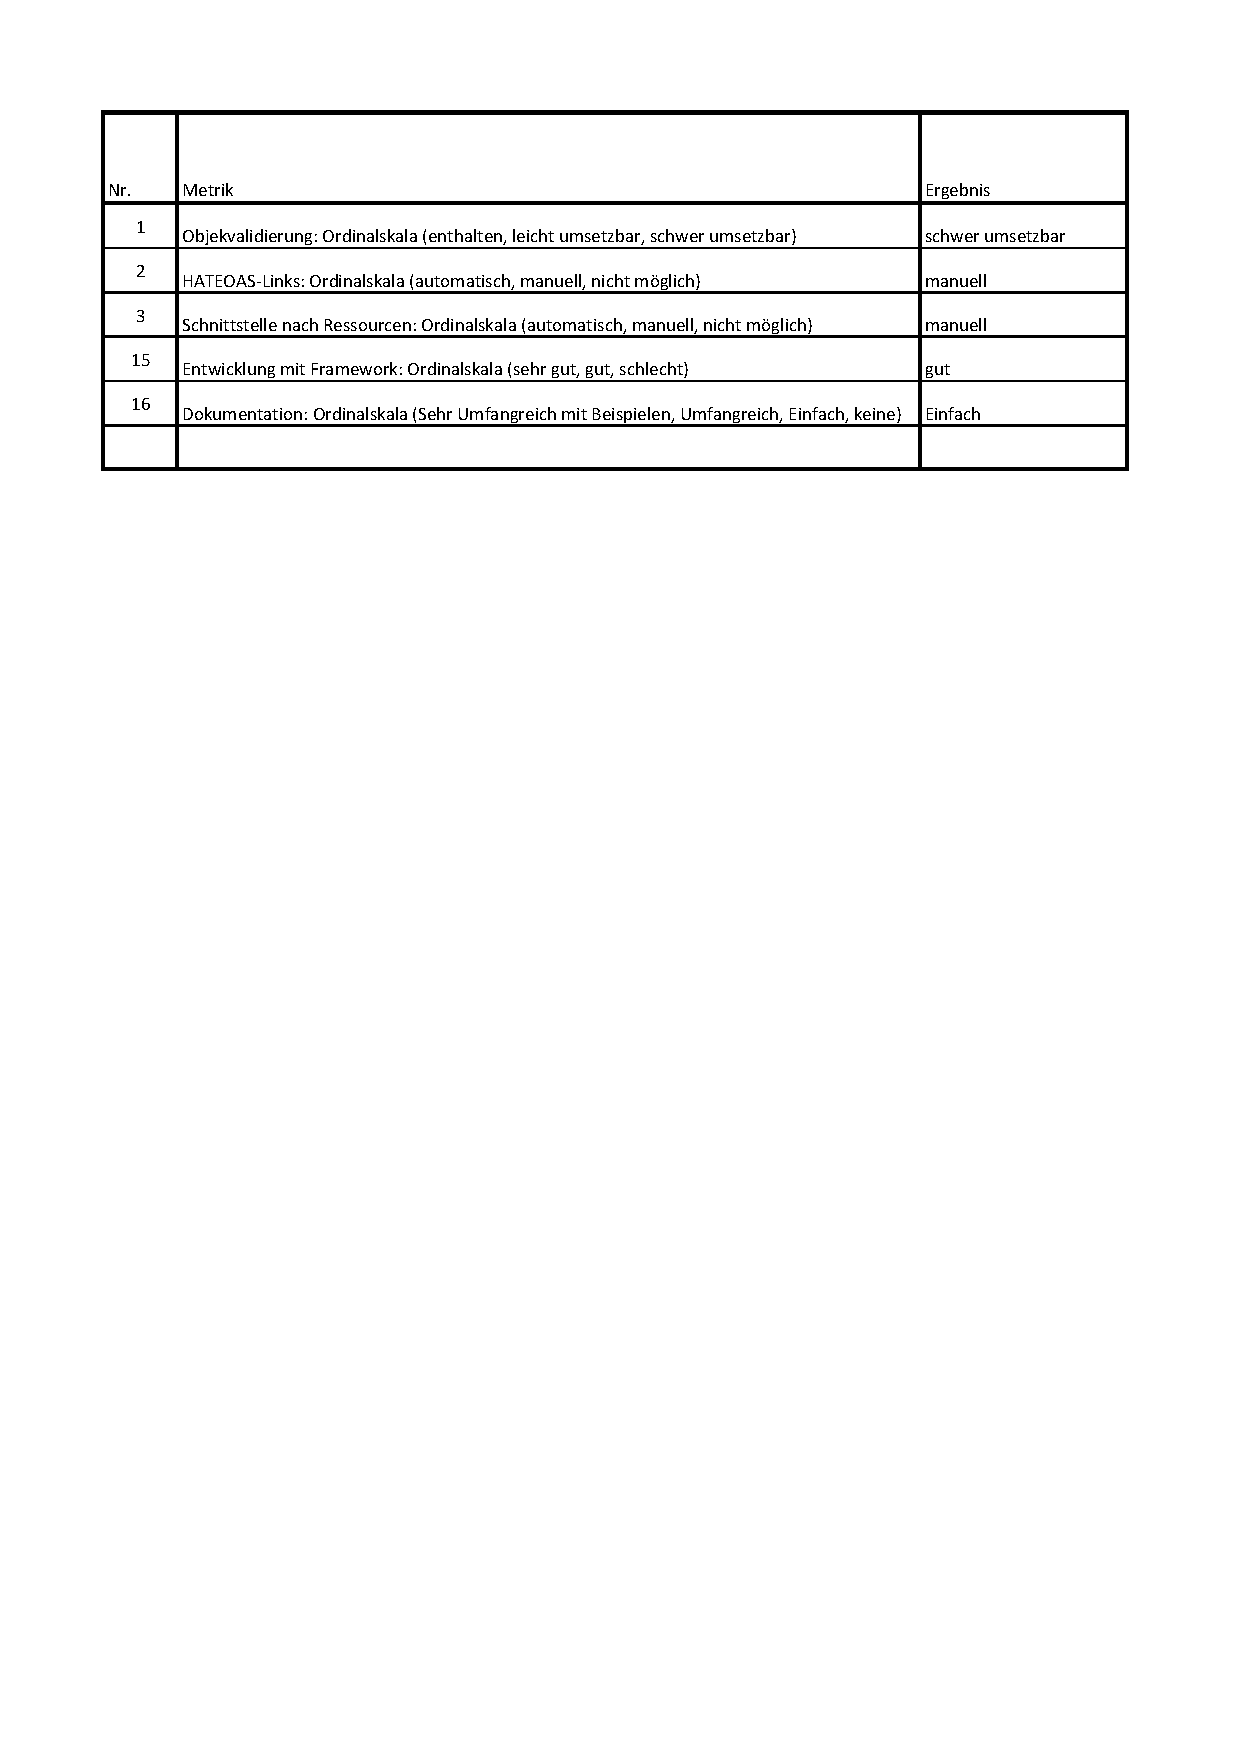
\includegraphics[width=\linewidth]{Bilder/Sz3ErgebnisGokit.pdf} \\	
	\caption[Szenario 3 Ergebnis GoKit]{Ergebnis von Szenario 3 für GoKIt}
	\label{Sz3ErgebnisGokit}\\
\end{longtable}
\FloatBarrier  

\newparagraph{Quantitative Evaluation}
Bei den Performance-Messungen konnte Go-Kit seine Stärken zeigen. Mit durchschnittlichen 9 Millisekunden Latenz kann der Service schnell Anfragen verarbeiten. So konnte er unter Last beachtliche 27.625 Anfragen/Sekunde beantworten und blieb dabei mit 31MB im Speicher sehr effizient\footnote{Für die Performance Messung wurde das Tool JMeter(\url{http://jmeter.apache.org}) eingesetzt und auf einem Laptop mit i7 2,3GHz Prozessor und 16GB DDR3 RAM durchgeführt.}.

Die Recherche bestätigte jedoch das bisher relativ schlechte Ergebnis. Obwohl das Framework auf der offiziellen Webseite als produktionsreif vermarktet wird\cite{GoKitFAQ2017}, steht es derzeit noch in Entwicklung und ist aktuell in der Version $0.3$ veröffentlicht. Somit gibt es zur Zeit weder einen offiziellen Support noch setzen, zu Recht, große Firmen auf dieses Framework.

Das Ergebnis der Quantitativen Evaluation ist in Tabelle \ref{QuantErgebnisGokit} dargestellt.  

\begin{longtable}{c}
	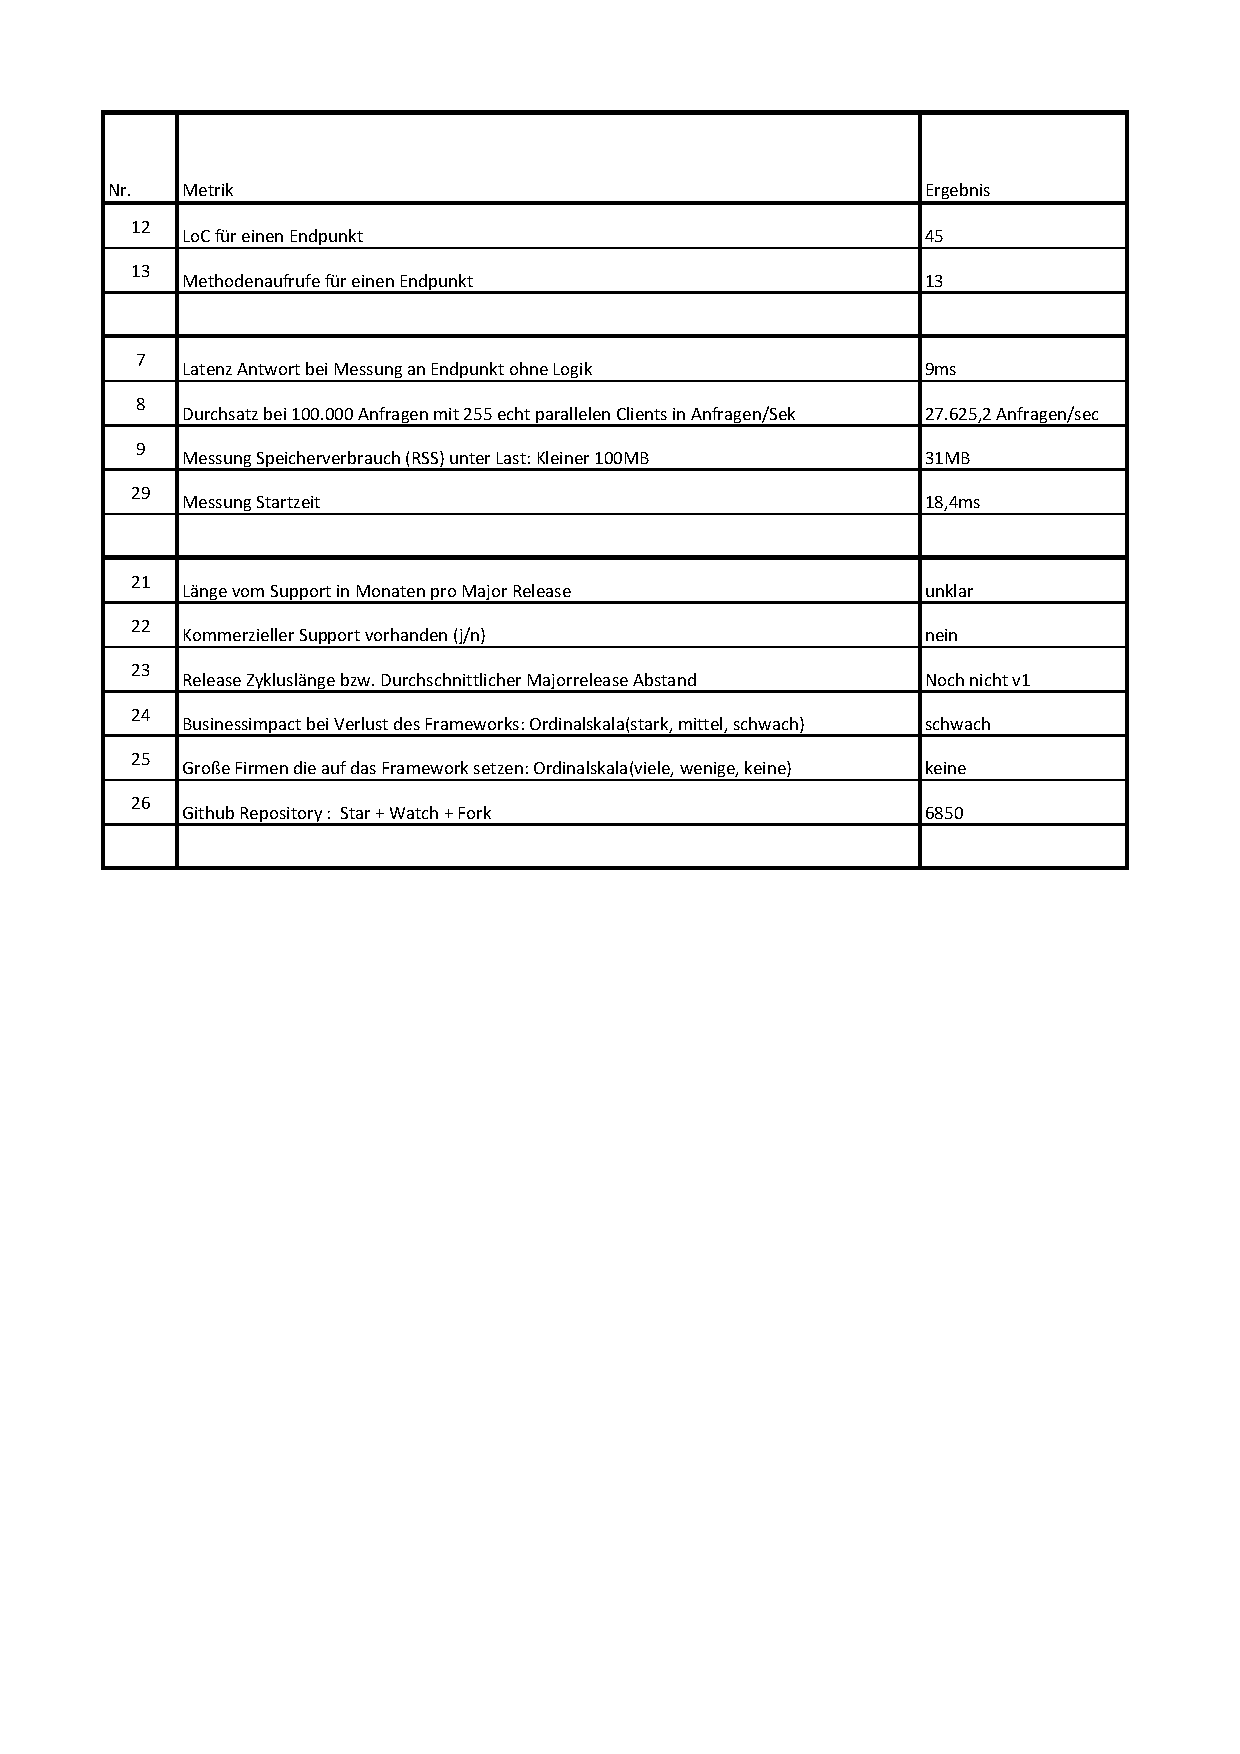
\includegraphics[width=\linewidth]{Bilder/ObjekEvalErgebnisGokit.pdf} \\	
	\caption[Quantitative Evaluation Ergebnis Go-Kit]{Ergebnis der quantitativen Evaluation von Go-Kit}
	\label{QuantErgebnisGokit}\\
\end{longtable}
\FloatBarrier

\subsubsection{Resümee Evaluationsphase}

Die Evaluationsphase ist die längste Phase von \ac{MFEM}. So hat die praktische Umsetzung der Szenarien und Messungen sowie die Einarbeitung in das Framework bei beiden Kandidaten eine Woche betragen. Aus diesem Grund ist es wichtig, bei der Ermittlung der Metriken auf die Prioritäten der Anforderungen zu achten. Wie bei der Evaluation von Go-Kit zu sehen war, hätte schon das Ergebnis des 2. Szenarios zu einem Abbruch führen können.\\
Durch die genaue Definition der Szenarien mit den zugehörigen Metriken erfolgt die Durchführung der Evaluation zudem sehr zielgerichtet. Mit etwas Disziplin kann so eine ausschweifende Entwicklung verhindert und somit der Zeitaufwand weitestgehend verkürzt werden. Hierzu sollten, wie von \ac{MFEM} vorgesehen, die Szenarien möglichst genau definiert werden.\\
Der Kreislauf zur Definition von Szenarien und der Zuordnung von Metriken hat sich in dieser Phase bewährt. So konnten keine Metriken übersehen und die Szenarien verfeinert werden.    

\subsection{Abschlussphase}

In der Abschlussphase werden die Ergebnisse aus der Evaluation aufbereitet und präsentiert. Aufgrund der Fülle von Anforderungen und erhobene Daten, wird dies hier nur exemplarisch an einer Qualitätskategorie für ein Framework durchgeführt. Die Auswertung der Restlichen erfolgt analog und findet sich als Excel Tabelle in den jeweiligen Github-Repositories sowie auf der beigelegten Daten-CD.

Die Aufbereitung der erhobenen Daten wird mit der komplexen Auswertung erfolgen. Die Abbildung \ref{AuswSpringWart} zeigt den kompletten Prozess.\\

\image[AuswertungSpringWartbarkeit.pdf][width=0.9\linewidth]{AuswSpringWart}{Auswertung Spring Wartbarkeit}{Auswertung und Zusammenführung aller Daten für die Qualitätskategorie \enquote{Wartbarkeit} am Beispiel Spring}

So wurden im ersten Schritt die ermittelten Ergebnisse auf einen Wert zwischen 0 und 1 normalisiert. Für die dreistufigen Ordinalskalen ergeben sich 3 mögliche Werte: $1$ für den höchsten, $0,5$ für den mittleren und $0$ für den niedrigsten Wert.\\
Bei den quantitativen Daten wird die prozentuale Abweichung zum Zielwert für die Normalisierung hergenommen. So ergab sich für die Supportlänge, mit einem Ergebnis von 10 und einem Zielwert von 12, ein Wert von $0,83$.
Die Erfüllung einer Ja/Nein-Frage kann wie eine zweistufige Ordinalskala angesehen werden. So wurde der vorhandene Support mit 1 normalisiert.\\
Nachdem die einzelnen Werte für eine Anforderung aufsummiert wurden, kann der prozentuale Erfüllungsgrad bestimmt werden. Bei 2 Anforderungen würde ein Wert von 2 einer vollen Erfüllung (100\%) entsprechen. Mit einem Wert von $1,5$ ergibt sich so ein Erfüllungsgrad von $87,5\%$.\\
Anhand der Prioritäten werden die Gewichte für die Zusammenführung der Anforderungen ermittelt. Eine mit \enquote{A} bewertete Anforderung geht vollständig in das Ergebnis über. Die Priorität \enquote{B} zählt zur Hälfte und \enquote{C} nur ein Viertel. So ergibt sich das Gesamtergebnis von $88,83\%$ für die Wartbarkeit von Spring.

Nachdem alle Ergebnisse aller Qualitätskategorien für Spring und Go-Kit mit diesem Schema ausgewertet wurden, konnte das Netzdiagramm erstellt werden. Abbildung \ref{FitnessVergleich} zeigt das Gesamtergebnis von Spring und Go-Kit in einer Grafik. 

\image[FitnessVergleich.pdf][width=0.9\linewidth]{FitnessVergleich}{Gesamtergebnis von Spring und Go-Kit}{Gesamtergebnis von Spring und Go-Kit als Netzdiagramm}
  
Das Gesamtergebnis macht die Überlegenheit von Spring deutlich. In nahezu jeder Kategorie hat es einen Vollausschlag. Lediglich bei der Performance kann Go-Kit Punkten. Aufgrund des miserablen restlichen Ergebnisses, wird jedoch auch dann von einem Einsatz im produktiven Umfeld abgeraten, falls die Geschwindigkeit ein maßgeblicher Faktor ist.\\
Der Einsatz von Spring ist dagegen sehr empfehlenswert, was der Erfolg und die weite Verbreitung des Frameworks zeigt.   

\subsubsection{Resümee Abschlussphase}

Die Auswertung der Daten ist sehr einfach und liefert ein ansehnliches Gesamtergebnis. Es kann dabei nur für sich stehen oder auch im Vergleich zu anderen Frameworks gut hergenommen werden, was die Abbildung \ref{FitnessVergleich} sehr gut zeigt. Auf dieser Basis kann schnell ein guter Überblick gewonnen werden, mittels dessen weitere Diskussionen durchgeführt oder Entscheidungen getroffen werden können.

\subsection{Gesamtauswertung \ac*{MFEM}}

Zusammenfassend kann gesagt werden, dass \ac{MFEM} seinen Zweck erfüllt. Die Diskrepanz, die bei der Wahl der Kandidaten eine Anforderung war, hat sich in den Ergebnissen widergespiegelt. So wurde trivialerweise ein gutes Framework äußerst positiv und ein unausgereiftes Framework negativ bewertet. Hierzu wurden, bis auf wenige Ausnahmen, nur die Basisanforderungen genutzt. So kann auch gesagt werden, dass diese bereits eine gute Grundlage für eine Bewertung darstellen.\\
Sämtliche Anforderungen lassen sich durch die Analysephase an die jeweilige Situation anpassen oder erweitern, sodass die Methode flexibel bleibt. Wie hier gezeigt wurde, entsteht so schnell eine Vielzahl an Anforderungen. Dazu bietet der Quality Utility Tree einen guten Ansatz, um den Überblick zu behalten und sich nicht in Feinheiten zu verlieren.\\
Die erste Hürde stellt die Wahl der passenden Metriken dar. Dies war auch bei dieser Evaluation durchaus eine Herausforderung. Auch wenn hier bis zuletzt kein Patentrezept für die Wahl der bestmöglichen Metriken ausgestellt werden kann, stellt die \ac{GQM} Methode einen guten Top-Down Ansatz dar, um dies zu unterstützen.

Bis zur Evaluationsphase, und selbst dort erst im letzten Schritt, spielt das eigentlich zu testende Framework keine Rolle. Dadurch bleibt die Methode sprachunabhängig und verkürzt sich bei mehrfacher Anwendung an verschiedenen Frameworks. Dieser Gewinn ist jedoch nur marginal, da die Durchführung der Evaluation am Framework den größten Zeitaufwand einnimmt. Hierzu bietet die Methode mit den Szenarien einen guten Ansatz, um den verhältnismäßig langen Prozess zumindest zielgerichtet zu gestalten. Wie sich gezeigt hat, kann durch die Priorisierung auch ein schneller Abbruch zustande kommen. So wird wenigstens nicht unnötig Zeit in einen negativen Kandidaten gesteckt.\\
Einzig die Abbruchbedingung wird von \ac{MFEM} nicht vorgegeben und sollte vor der Durchführung definiert werden. Eine Bedingung im Zusammenhang mit den Prioritäten ist hierfür prädestiniert.

Das mittels Netzdiagramm dargestellte Gesamtergebnis bietet einen sehr guten und schnellen Überblick über das Ergebnis. So kann der Architekt auch vor nicht allzu technisch versierten Entscheidungsträgern seine Wahl anschaulich begründen, ohne zu tief ins Detail gehen zu müssen.     














\pagebreak

% ----------------------------------------------------------------------------------------------------------
% Zusammenfassung
% ----------------------------------------------------------------------------------------------------------
\section{Vergleich und Ausblick}
\subsection{Methoden Anpassung/Erweiterung}
\subsection{Ausblick}


\pagebreak

% ----------------------------------------------------------------------------------------------------------
% Literatur
% ----------------------------------------------------------------------------------------------------------
\renewcommand\refname{Quellenverzeichnis}
\bibliographystyle{myalpha}
\bibliography{bibo}
\pagebreak

% ----------------------------------------------------------------------------------------------------------
% Anhang
% ----------------------------------------------------------------------------------------------------------
\pagenumbering{Roman}
\setcounter{page}{1}
\lhead{Anhang \thesection}

\begin{appendix}
\section*{Anhang}
\phantomsection
\addcontentsline{toc}{section}{Anhang}
\addtocontents{toc}{\vspace{-0.5em}}

\section{CODE}
Nothing Here

\end{appendix}
\end{document}
